%% 2016/07/25
%% by Sylvain Chatel
%% See:
%% sylvain.chatel@supelec.fr
%% Report paper on the cyber security of the distributed model predictive control

%% This work is distributed under a CC-BY License.
%%*************************************************************************

%% PH : remarque sur la méthode de compilation. Je crois que tu as utilisé latex -> DVI ->.... -> PDF. Il faut mieux utiliser ``pdflatex'' qui compile directement en PDF (pas de DVI, pas de PS). C'est plus simple et je crois que ça passe aussi mieux pour les images.


\documentclass[conference]{IEEEtran}
\usepackage[utf8]{inputenc}
\usepackage[T1]{fontenc}
% \usepackage[francais]{babel}
\usepackage{graphicx}
\usepackage{mathrsfs}
\usepackage{color}
\usepackage{colortbl}
\usepackage{amsfonts}
\usepackage{amssymb}
\usepackage{graphicx}
\usepackage[top=2cm, bottom=2cm, left=2cm, right=2cm]{geometry}
\usepackage{mathrsfs}
\usepackage{textcomp}
\usepackage{nccmath}
\usepackage{pgf}
\usepackage{float}
\graphicspath{{figures/}}
\usepackage{stmaryrd}
\usepackage{bm}

% *** CITATION PACKAGES ***
%
\usepackage{cite}

% *** MATH PACKAGES ***
%
\usepackage{amsmath}

% *** ALIGNMENT PACKAGES ***
%
\usepackage{array}

% correct bad hyphenation here
\hyphenation{op-tical net-works semi-conduc-tor}
\edef\hc{\string:}

% Remarques dans le texte en bleu:
\newcommand{\rem}[1]{\textcolor{blue}{[#1]}}

\begin{document}
%
\title{Security of the Distributed Model Predictive Control }


% author names and affiliations
% use a multiple column layout for up to three different
% affiliations
\author{\IEEEauthorblockN{Sylvain Chatel, Pierre Haessig and Romain Bourdais.}
\IEEEauthorblockA{CentraleSupélec - IETR - UMR 6164, France\\
Email: sylvain.chatel@supelec.fr, $\{$pierre.haessig ; romain.bourdais$\}$@centralesupelec.fr
}
}

% make the title area
\maketitle
\thispagestyle{plain}
\pagestyle{plain}

\begin{abstract}
In this paper, we explore the security of a distributed model predictive control (DMPC) scheme. A global system is decomposed into several local subsystems \rem{which share a common ressource...}. Each subsystem has a model predictive control (MPC) controller which cooperates and works iteratively with all the other controllers through a coordinator in order to reach the global objective of the system. Here, we focus on the security of such a system. Indeed, we report that a user can disturb the DMPC through several attacks in order to destabilize the resource distribution. Hence, examples of cheating protocols and counter-cheat ideas are presented and discussed.
\end{abstract}


PH: {\itshape l'abstract est bien concis. Deux remarques :
\begin{itemize}
  \item écrire au présent (j'ai corrigé ici, mais ça concerne aussi tout l'article)
  \item mieux préciser le \emph{contexte} : ``subsystems are sharing a common ressource (e.g. heating power)...''. C'est cela qui justifie le \emph{besoin de coordination}.
\end{itemize}
}


\section{Introduction}
Model predictive control (MPC), also known as \textit{receding horizon control}, is becoming more and more popular in the industrial process control \cite{Venkat, Campo}. Among other benefits \rem{j'ai fait une recherche de ``perks'' et il semblerait que ce soit plutôt un avantage dans un contexte professionnel}, the attractiveness of the MPC lies in its ability to represent clearly the constraints of the optimization problem \cite{Jia}. Over the past decades, the MPC has become widespread and many successful applications have been developed in the process industry.

In MPC, the objective is to get the optimal control input over a given horizon by solving a discrete-time optimal control problem. Traditionally, this kind of control is done by a controller in a centralized way.  This controller has full knowledge of the system behaviour over the horizon. Although efficient, this schemes might sometimes be inadequate. For instance,  for large-scale interconnected systems such as power and water distribution or even traffic systems (with plug and play), a centralized MPC might not be ideal or even technically feasible \cite{Jia}. Moreover, the fact that the controller is omniscient and  fully knowledgeable might be an obstacle because some agents might not be able or willing to divulge information about their local subsystem. This might be the case as \cite{Campo} points out for the newly regulated power markets in the United States.

These two issues of scalability and privacy motivate the choice of a distributed MPC architecture. The global system is decomposed into several subsystems. Each subsystem has a MPC controller which communicates with the others. Local control inputs are then locally computed and determined with the few information shared. For instance, when a decentralized control scheme (where local control input are determined based on local measurements for instance) is needed, a distributed MPC is a better choice. For example, for water distribution systems, a centralized MPC is decomposed into a DMPC using a coordinator (e.g. augmented Lagrangian \cite{Campo} or Uzawa method \cite{Cohen}).

\rem{ici préciser ou dans les paragraphes suivants que la méthode de distribution dépend du \emph{type de dépendance} entre les subsystems.
Préciser aussi le type de dépendance qui nous intéresse : la ressource partagée}.

Several distributed MPC examples are available in the literature. DMPC frameworks were developed in \cite{Acar, Sawa} and \cite{ Dunbar}. In the latter \rem{je ne sais pas si latter marche aussi quand il y a plus que 2 objets}, a MPC framework is developed for a system with several independent subsystem dynamics but nonetheless linked through their cost functions. \rem{là on aimerait en savoir un peu plus sur 5 et 6...}

In a DMPC, each agent communicates with the others via a simple coordinator. This latest, returns a simple information (e.g. a Lagrangian multiplier for an augmented Lagrangian technique). All the information required for the system to work efficiently is communicated through this small amount of data. As pointed out by Brooks \emph{et al.} \cite{Brooks}, though efficient, DMPC still suffers from some risks. Indeed, DMPC might sometimes be harmful to the physical system. For instance in a complex system \rem{ajouter ``like a power grid'' ? }, human error, malicious and misleading agents could easily disturb the grid. According to Brooks \emph{et al.}, one of the best ways to mitigate those security threats is to involve a combination of counter measures such as using fault detection softwares, limiting the size of each entity or even certifying aggregators. However, to the best of our knowledge, there has been no comprehensive study on security threats and counter measures at the level of DMPC \emph{algorithms} (as opposed to the lower level layers like communication protocols).
This article is a first attempt to start filling this gap \rem{phrase un peu moyenne, si tu as une meilleure idée...}.

The paper is organised as follow.  Section II introduces the model of DMPC for power distribution used in our study. In Section III,  a study of the base cases is conducted. The security threats are implemented and studied in section IV. In Section V, the main contributions of this study are summarized.


\section{Model}

PH: {\itshape
la modélisation est assez claire. Qq points en particulier sur les  notations:

\begin{itemize}
  \item expliquer le sens du critère Ju: minimiser l'énergie, avec une contrainte soft (cad une pénalisation des écarts) sur la température.
  \item ajouter les indices "i" dans les équations pour R et C, et aussi sur fig 1.
  \item Corriger "U" en "u" sur fig. 1 et 2.
  \item clarifier le rôle de "k": est-ce le temps de la simulation ou le temps de l'horizon MPC. Clarifier de même la défintion des vecteurs "U" et "X" majuscules.
  \item utiliser une autre lettre que k pour l'indice d'Uzawa, sinon on s'en sortira pas (ou inversement utiliser indice t pour le temps, ça se fait parfois).
  \item utiliser \emph{eqref} plutôt que \emph{ref} pour référencer des équations. ça ajoute des parenthèses.
\end{itemize}
}

In this paper, we consider a linear time-invariant (LTI) system composed of $m$ interconnected subsystems. Each subsystem represents a room with a thermal capacity $C_{th}$ and a thermal resistance to the outside $R_{th}$, as depicted on figure \ref{thermmod}.
Taking into account the exterior temperature $T_{ext}$, the objective is for the temperature of each room $T_i$ to be as close as possible to an ideal reference temperature $T_{id}^i$ at each time. All rooms are getting their energy from a limited \emph{global} amount of energy\rem{energy-> power à bcp d'endroits} $U_{max}$, and each user has a \emph{local} maximum  admissible energy $u_{max}^i$ due to its physical configuration. We note $u_i$ the energy consumed by user i. Since the consumed energy cannot exceed the maximum admissible energy, and since the global energy resource is limited, we have the first two constraints :

\begin{equation}
\forall i \in \llbracket 0, m-1 \rrbracket, \; 0 \leq  u_i \leq  u_{max}^i 
\label{uimax}
\end{equation}

\begin{equation}
\sum_{i = 0}^{m-1} u_i \leq U_{max}
\label{umax}
\end{equation}

\rem{Main objective is to min. energy ...}. Then, in order to take into account the will of each user to reach its ideal temperature, we introduce a comfort factor $\alpha$.  Hence the optimization problem is to minimize the following cost function subjected to \ref{uimax} and \ref{umax}.

\begin{equation}
J_u = \sum_{i = 0}^{m-1} u_i  \; + \; \sum_{i = 0}^{m-1} \alpha_i (T_i - T_{id}^i)^2 
\label{cost}
\end{equation}

In order to determine the $J_u$, we used the thermal model presented in Figure \ref{thermmod}.

\begin{figure}[!t]
\centering
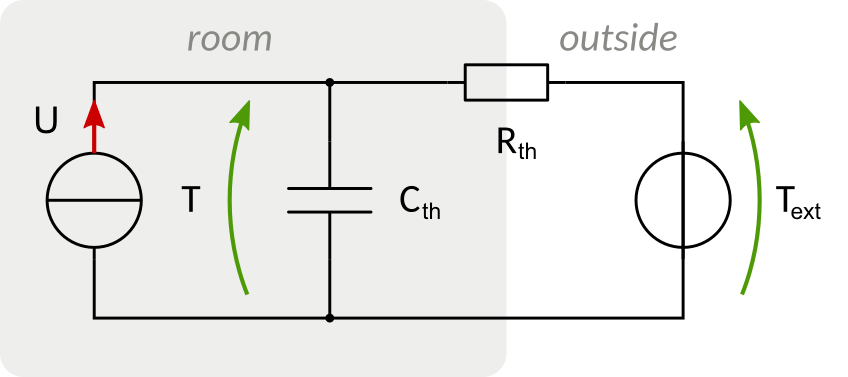
\includegraphics[width=3in]{therm_diagram.png}
\caption{Thermal model of a room. $R_{th}$ represents the thermal resistance and $C_{th}$ the thermal capacity of the room. $U$ is the consumed power, $T$ the temperature of the room and $T_{ext}$ the external temperature.}
\label{thermmod}
\end{figure}

With this model, it is possible to use the state-space representation of the problem. We can  set $\bm{X}[k]$ as the temperature vector of each room. $\bm{U}[k]$ represents the consumed energy of each room and $\bm{U}_{ext}[k]$ the external temperature. 
With those notations, we can write:

\begin{equation}
\bm{X}[k+1]\; = \; A . \bm{X}[k] + B .\bm{U}[k] + B'.\bm{U}_{ext}[k]
\label{state}
\end{equation}

Given equation \ref{state}, and the model, we can replace the temperature in equation \ref{cost}. This enables us to have a quadratic problem in $\bm{U}$ :

\begin{equation}
J_u = \bm{U}^T P \bm{U} + q^T \bm{U} + cst 
\label{cost_en}
\end{equation}

In order to proceed to a centralized MPC, we have to minimize \eqref{cost_en} subject to \eqref{uimax} and \eqref{umax}. However, in order to have a distributed MPC, we need to decompose the computation to all users. To this end, we used an Uzawa method. The idea is to relax the constraint which couples local decisions, that is the global constraint \eqref{umax}. A Lagrange multiplier $\lambda$ associated to \eqref{umax} is introduced, and it is managed by a central \emph{coordinator}. After being initialized (at 0), the coordinator dispatches $\lambda$ value to each subsystem. Then each subsystem can proceed independently to the minization of its local objective \rem{formule de l'objectif local pénalisé par $\lambda$ à ajouter}. The coordinator collects the result of these local minization and updates the multiplier acording to a gradient ascent formula:
\begin{equation}
\lambda_{k+1} = \lambda_k + p  \left(\sum_{i=0}^m u_i^*[k] - U_{max} \right)
\label{lambda}
\end{equation}

\rem{choisir: soit ``[k]'' soit ``indice k'' mais pas les deux!}

where $p$ represents the step of the gradient ascent and $u_i^*[k]$ the optimal consumption of user $i$ at iteration $k$. This iterative procedure is done until the difference between $\sum_{i=0}^{m-1} u_i^*[k]$ and  $U_{max}$ is lower than a threshold $\varepsilon$ \rem{donner plus loin sa valeur dans les expériences}. We note $\lambda_{opt}$ the value of the multiplier fulfilling this condition.

\begin{figure}[!t]
\centering
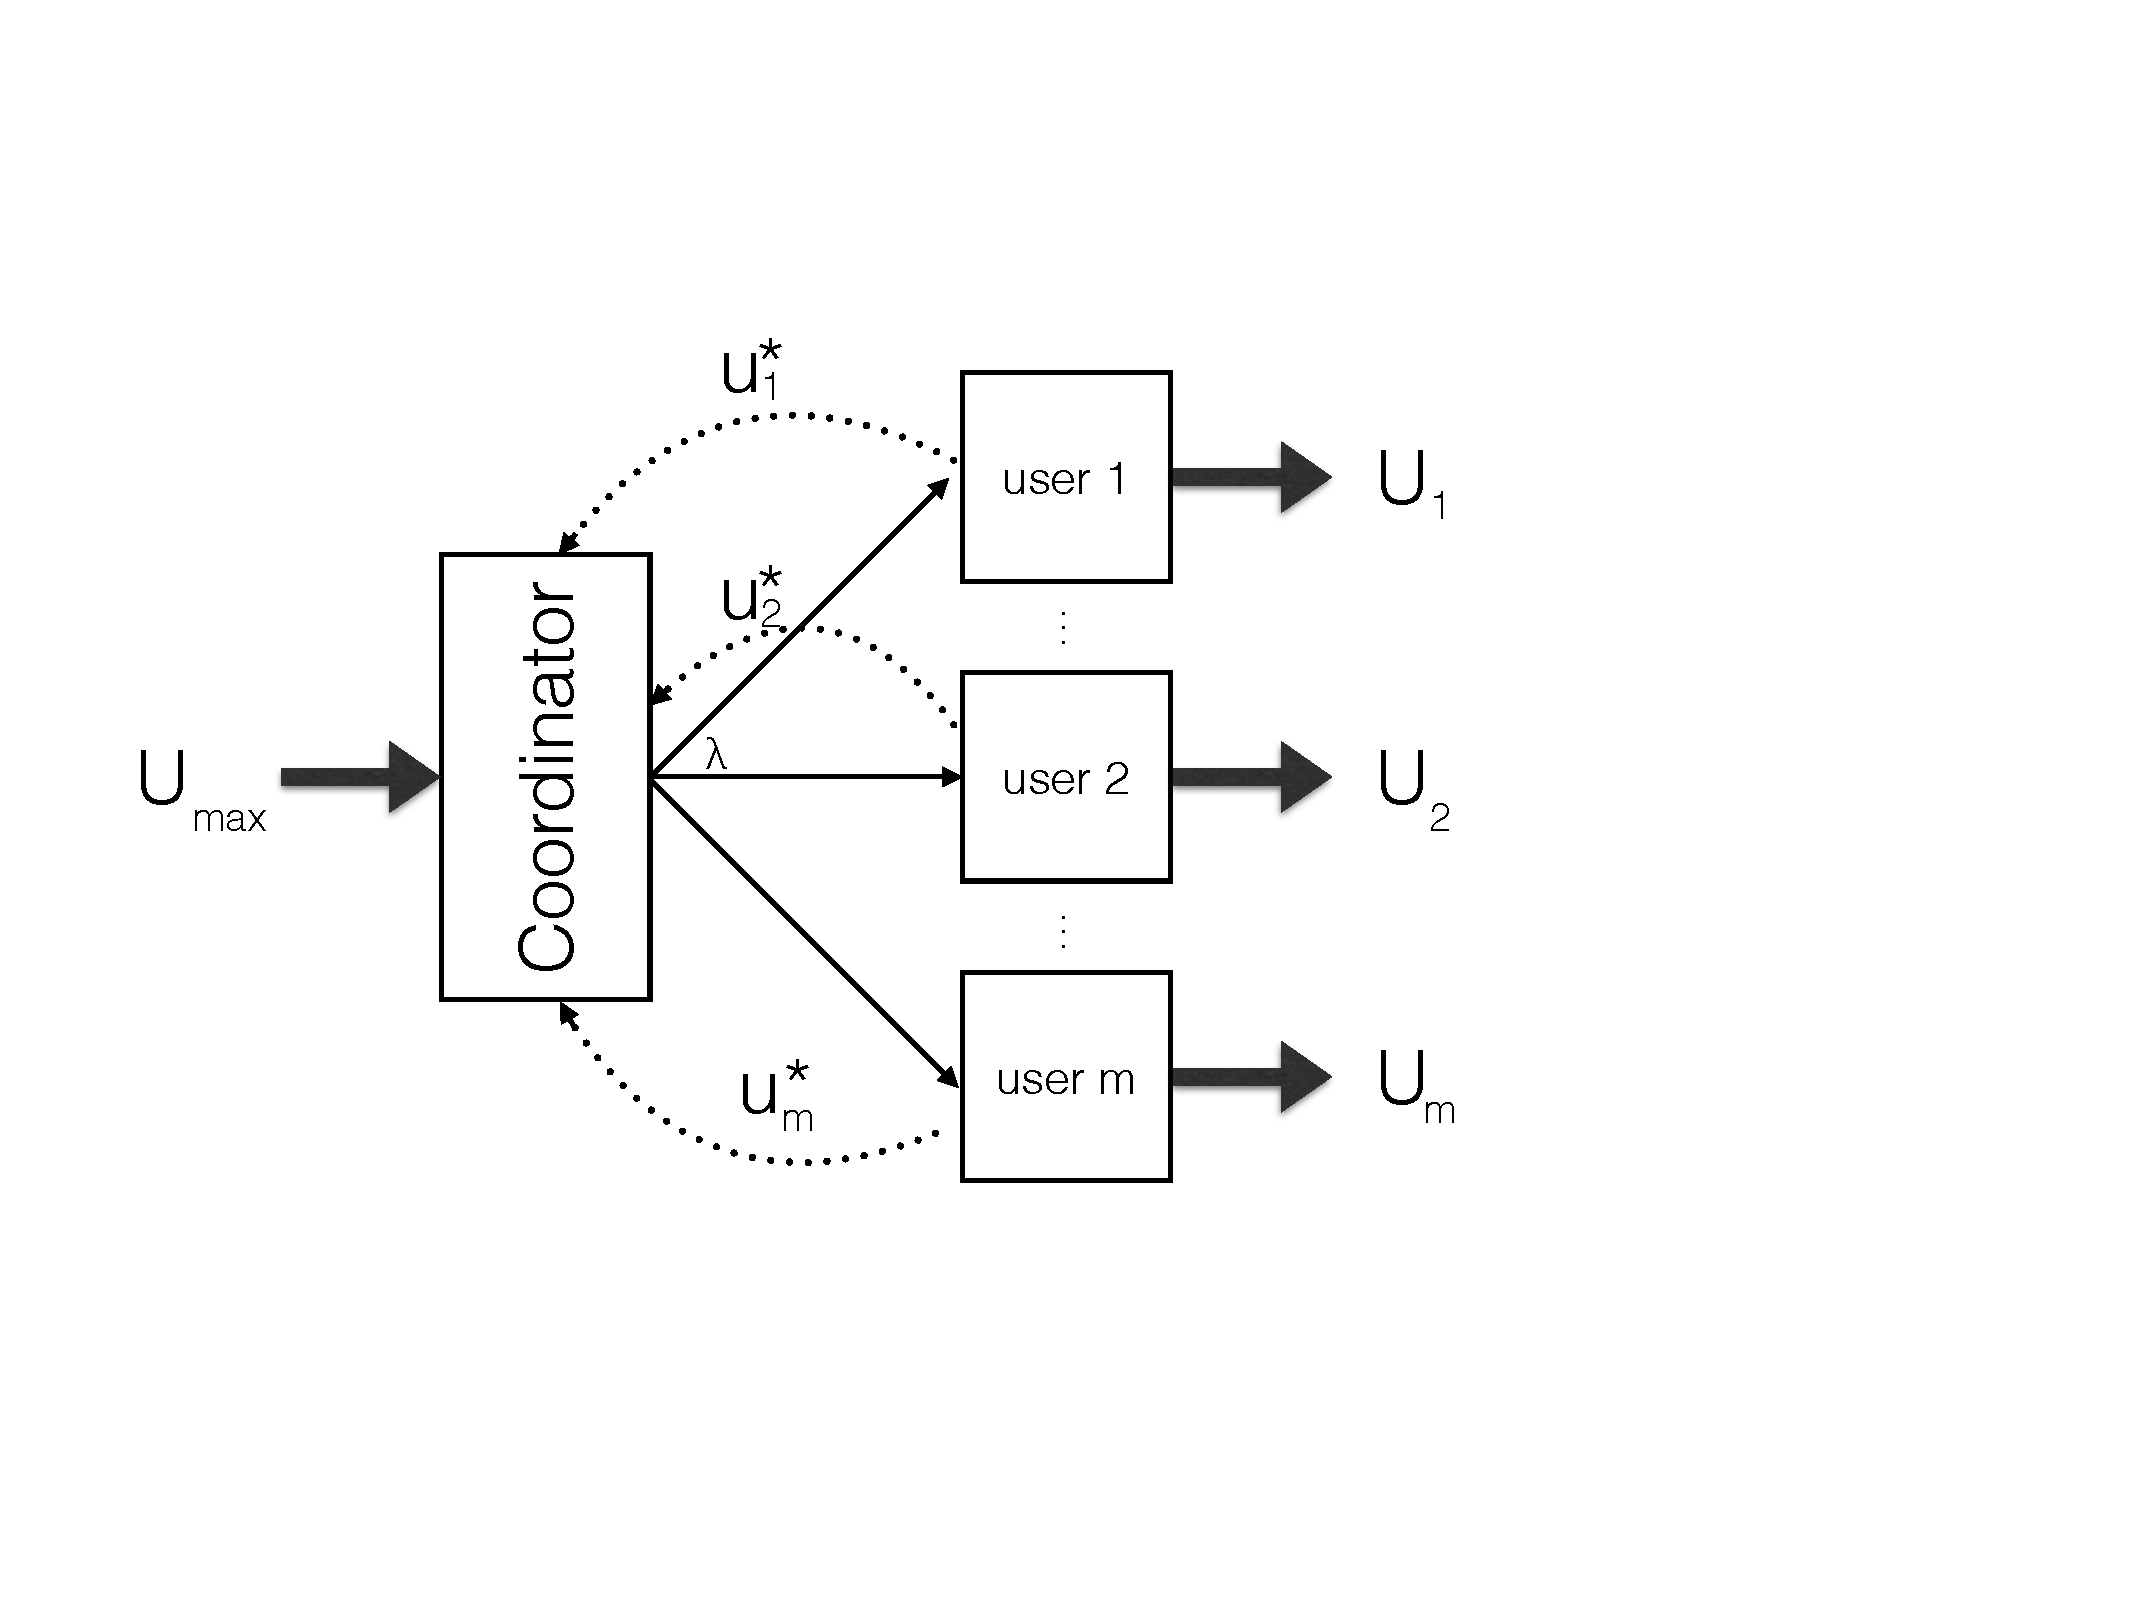
\includegraphics[width=3in]{ASHschema}
\caption{Structure of the distributed problem}
\label{coord}
\end{figure}
To summarize, the DMPC requires to solve the following quadratic problem over a prediction horizon $N$ for a simulation lasting over $N_{sim}$ \rem{attention, là on parle de temps, mais la plupart des équations précédentes sont statiques. Peut-être que le texte précédent correspond à une subsection II.A "static case", et qu'il faut ensuite II.B "dynamic" qui explique le MPC.
Préciser aussi que dans le cas dynamique, $\lambda$ est un vecteur.} :
\begin{equation}
\left\{
\begin{array}{l}
\text{min} \; J_u[j] =   \bm{U[j]}^T P \bm{U}[j] + q^T \bm{U}[j] + cst[j] + \lambda[k_{opt}]  \\
\text{subjected to}\\
\forall j  \in \llbracket 0, N_{sim}-1 \rrbracket, \forall i \in \llbracket 0, m -1 \rrbracket, \; 0 \leq  u_i \leq  u_{max}^i
\end{array}
\right.
\label{QP}
\end{equation}

In our case study, we opted for $N_{sim} = 24$ h \rem{N est un entier sans dimension. Formulation alternative :}. In our study, we simulate 24 hours, which is $N_{sim} = 240$ points with a time step $\Delta_t=0.1$ h.


\section{Base cases}
In this section, we present the results for the nominal experiment of power distribution in several cases : the static case, the centralized dynamic case and the distributed dynamic case. All those simulations were made via the python module we developed. This package relies on \texttt{cvxopt} package \rem{ajouter un cite vers une entrée bibtex avec pour titre `` CVXOPT: Python Software for Convex Optimization'' une url, num version, et les 3 auteurs (Dahl était manquant)} for convex optimization \cite{Boyd}.

{\itshape Commentaire général sur les expériences :

\begin{itemize}
  \item donner toutes les données de chaque expérience (en texte ou en tableau)
  \item bien \textbf{décrire ce qui est doit être vu} sur chaque figure,
  en commençant du plus simple/évident pour aller avec le plus
  subtil. Expliquer en particulier qui est uid
  \item font trop petite sur la pluspart des graphs. Pour la légende je suppose que c'est assez galère pour la mettre à l'extérieur. Je pense que c'est plus rapide de jouer avec
  le param \texttt{location}. Par exemple "lower right" pour les graphs à barres.
\end{itemize}

}
\subsection{Static case}

\rem{bien expliquer là (ou avant au §II): 1) qu'est-ce que ce static case, et 2) pourquoi on l'étudie}

\subsubsection{Centralized case}



Let us consider a problem with three different users. We consider, at first, that all users are identical. We set the system so that $U_{max}$ is inferior to the sum of all admissible temperature. 
\begin{figure}[H]
\centering
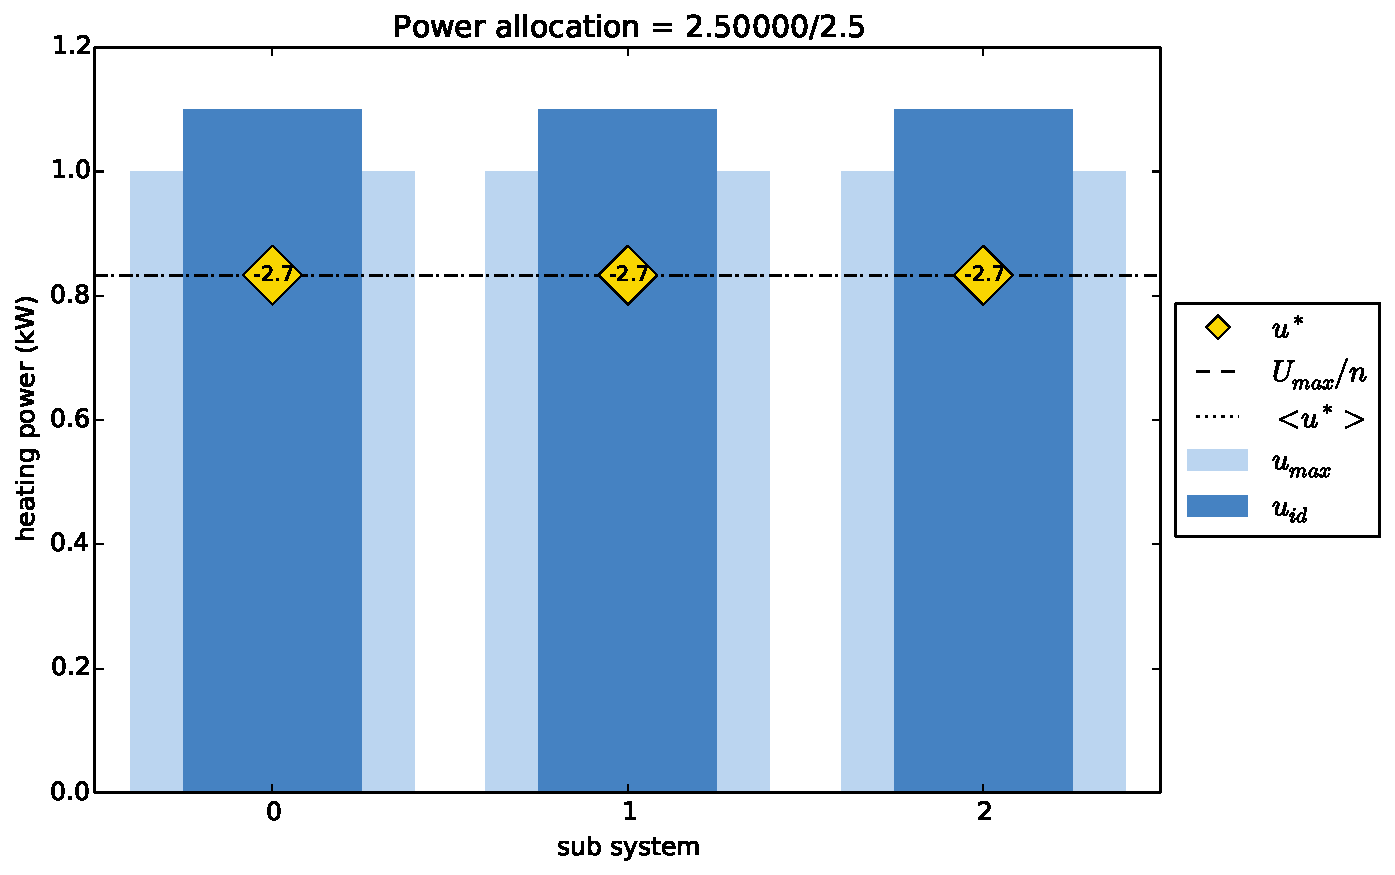
\includegraphics[width=3in]{static_PB_init.pdf}
\caption{Optimal power distribution in a static symmetrical case
\rem{voir remarque sur la cohérence des expériences fig 14.}
}
\label{statPBinit}
\end{figure}

Now, if we change the comfort factor of the third user in order for him to be more comfortable. To do so, let us take $\alpha_2 = 10\times  \alpha_0 $.

\begin{figure}[H]
\centering
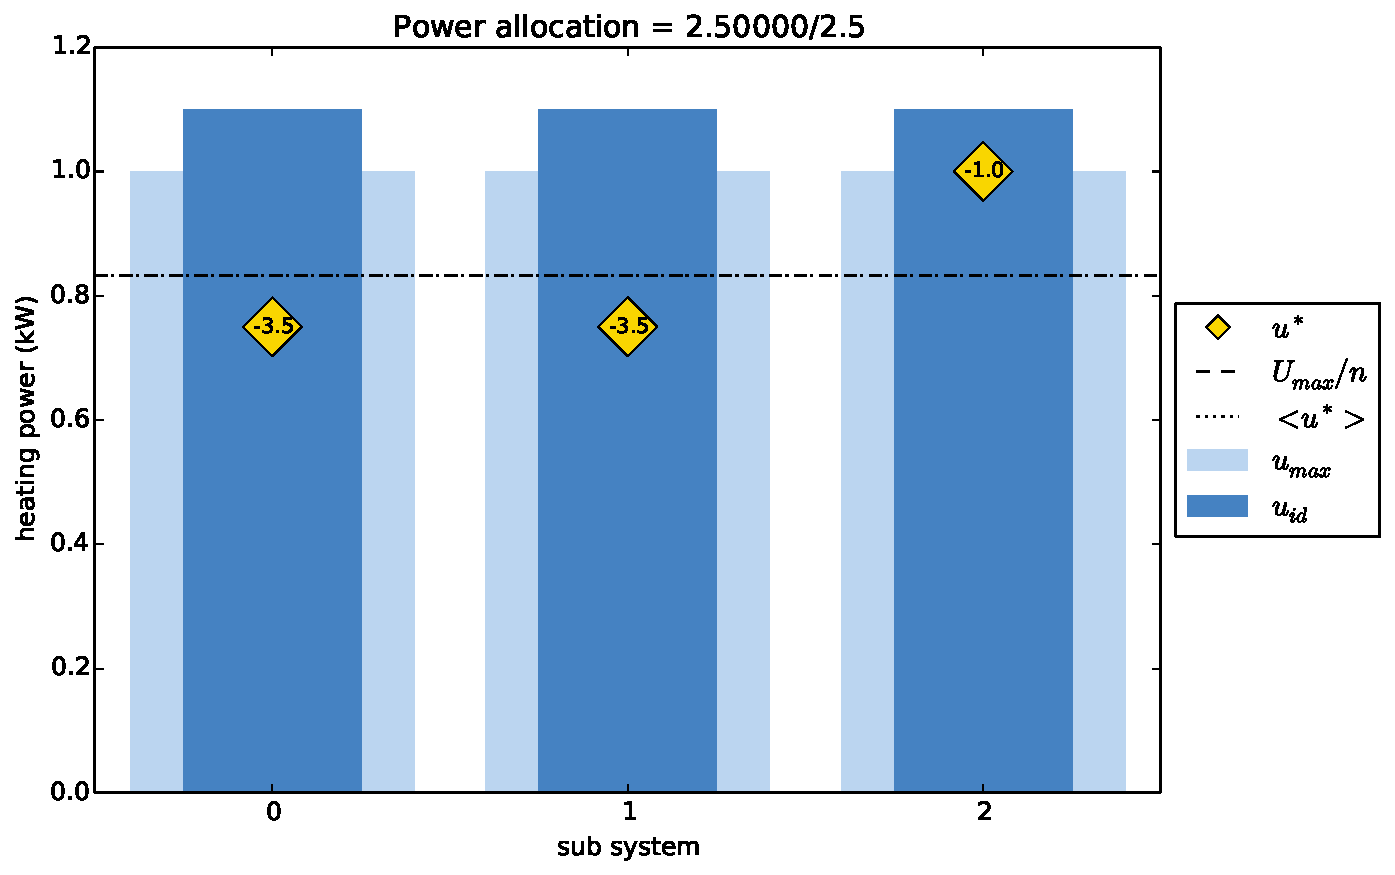
\includegraphics[width=3in]{static_PB_cht.pdf}
\caption{Optimal power distribution in a static case with different priorities, $\alpha_2 / \alpha_0 = 10$}
\label{statPBcom}
\end{figure}

When comparing Figure \ref{statPBinit} and \ref{statPBcom}, we notice that the user 2 is indeed preferred in the power distribution and then its comfort becomes better to the disadvantage of the others (i.e. the square deviation to the ideal temperature of user 2 is the smallest of all users \rem{enlever l'embrouille ``third'' vs. ``number 2'' dans le reste du texte aussi}.

\subsubsection{Distributed case}
When we decompose the centralized computation with the Uzawa method, we are able to model a distributed optimization. At first we consider a symmetrical situation.  

\rem{allégement possible : ne garder qu'une des deux expériences. le point clé est ici de montrer que Uzawa permet d'obtenir le même résultat que le centralisé, à une tolérance près. Pas besoin de le montrer deux fois.}

\begin{figure}[H]
\centering
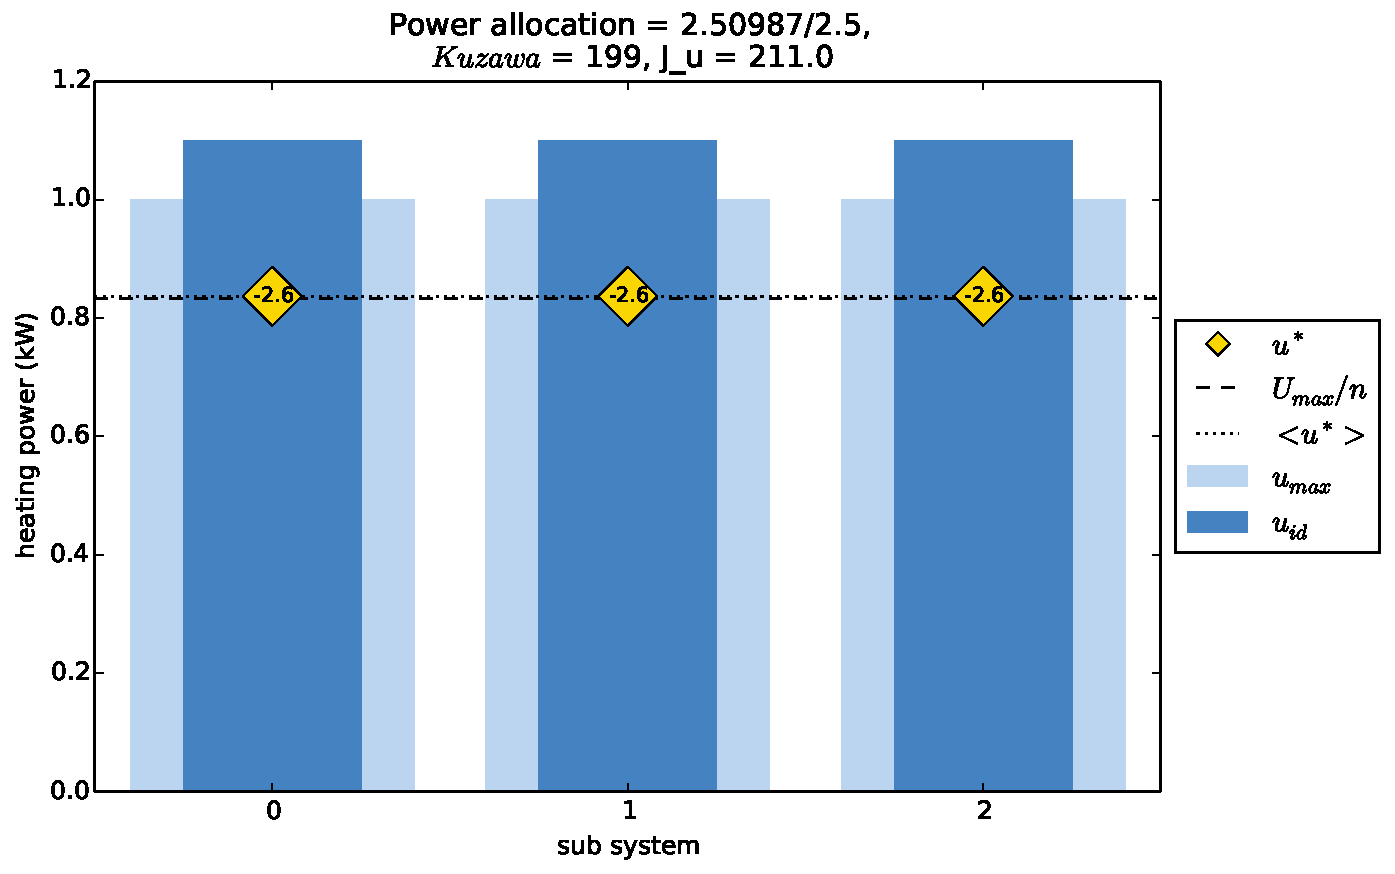
\includegraphics[width=3in]{static_DPB_init.pdf}
\caption{Optimal power distribution in a static symmetrical distributed case}
\label{statDPBinit}
\end{figure}

Now, if we change the comfort factor of the third user in order for him to more comfortable. To do so, let us take $\alpha_2 = 10 \times \alpha_0 $.

\begin{figure}[H]
\centering
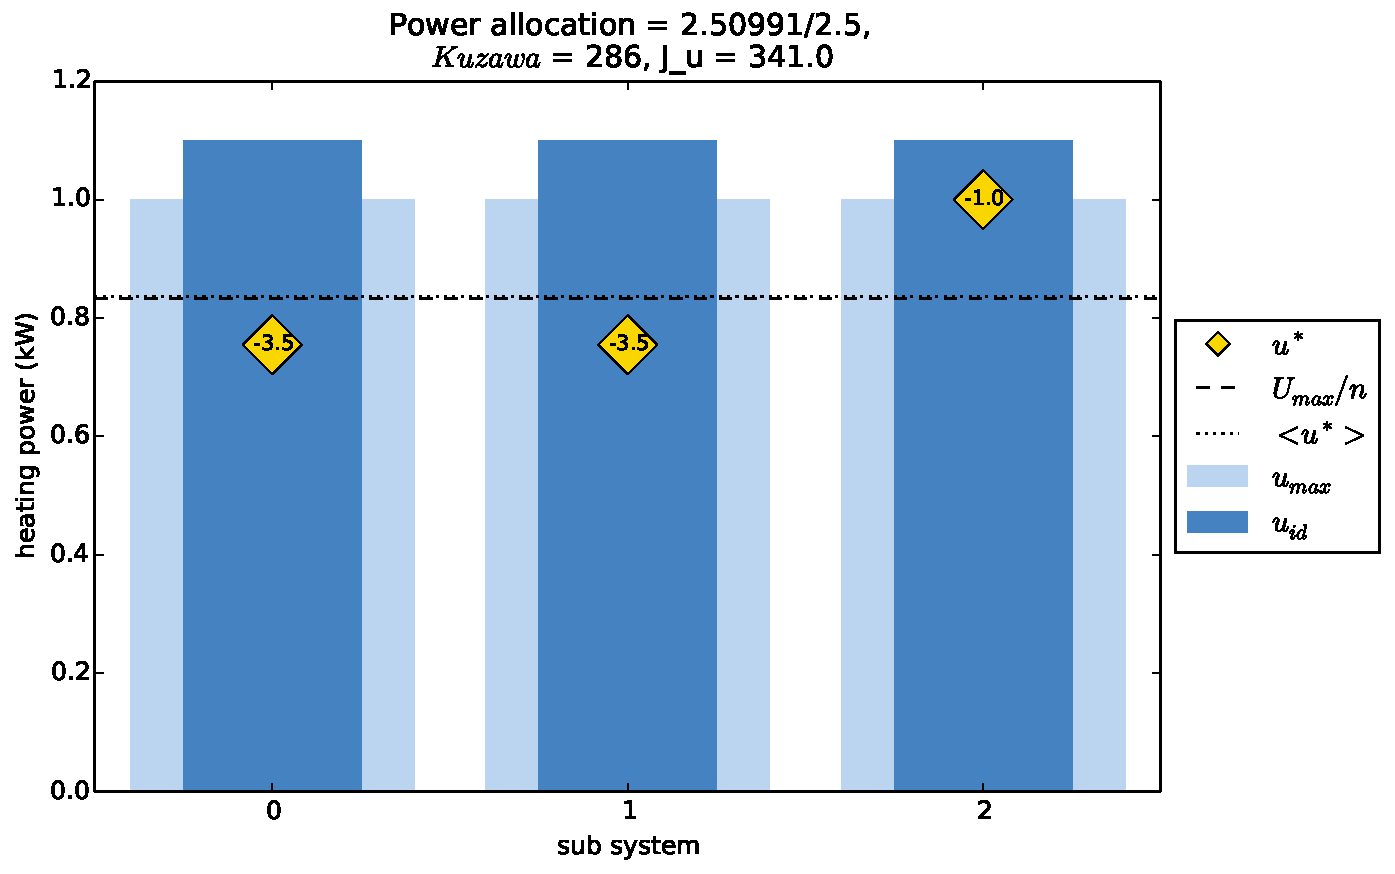
\includegraphics[width=3in]{static_DPB_cht.pdf}
\caption{Optimal power distribution in a static distributed case with different priorities, $\alpha_2 / \alpha_0 = 10$}
\label{statDPBcom}
\end{figure}
 
 When comparing Figure \ref{statDPBinit} and \ref{statDPBcom}, we notice ``as before'' \rem{comme tu le dis, c'est redondant!} that the third user ($n^{\circ}2$ is more satisfied to the disadvantage of user 1 and 2. We notice as well that the total amount of consumed energy is superior to $U_{max}$. This phenomenon is due to the constraint relaxation executed in the Uzawa method.
 
 Through this nominal static study, we were able to determine the influence of all the different parameters on the optimal solution among which the Uzawa step determination in order to have a convergence of the Uzawa iteration \rem{phrase un peu trop compliquée}.  We then used those results in the study and set $p = 1.5$. \rem{un graph montrant la convergence de la violation de contrainte pour différents choix de $p$ serait un plus.}.
 
 \subsection{Dynamic case}

 \rem{comme pour le cas statique, donner la valeur de tous les parmètres. y compris Tout}

 Now, we consider a dynamic simulation on a horizon of 24 hours. Three different users are using a limited amount of energy $U_{max}$\rem{= ...}. The ideal temperature is determined with a time based profile: between 6\hc 30-8\hc 30 am and 18\hc 00-22\hc 00 pm the user wishes to have a temperature $T_{pres}$\rem{= ...} (people are present in the room), the rest of the time the temperature is set to $T_{abs}$\rem{= ...}.
 
\begin{figure}[H]
\centering
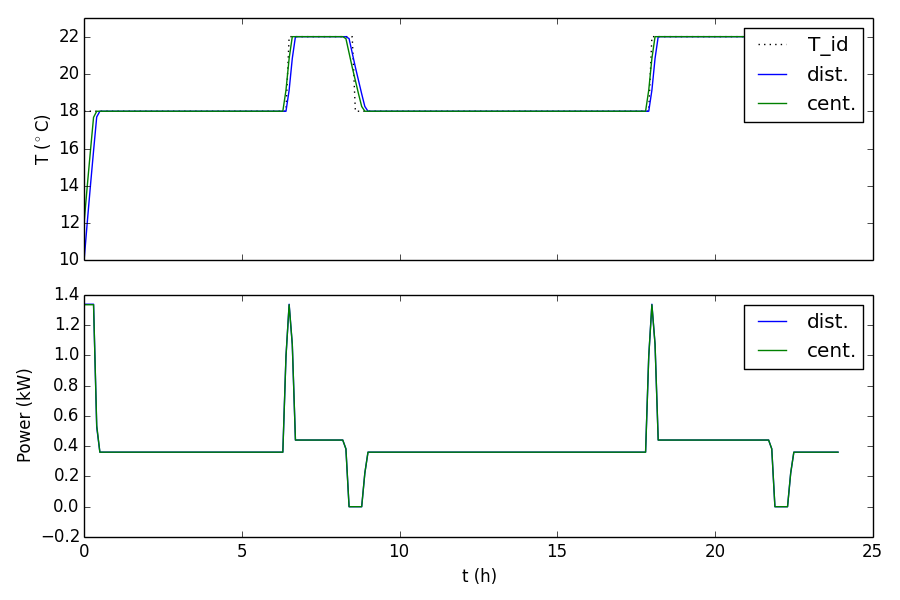
\includegraphics[width=3in]{dynDMPC_init.png}
\caption{Optimal power distribution in a dynamic case for user 2 in a symmetrical problem}
\label{dynDPBinit}
\end{figure}
\begin{figure}[H]
\centering
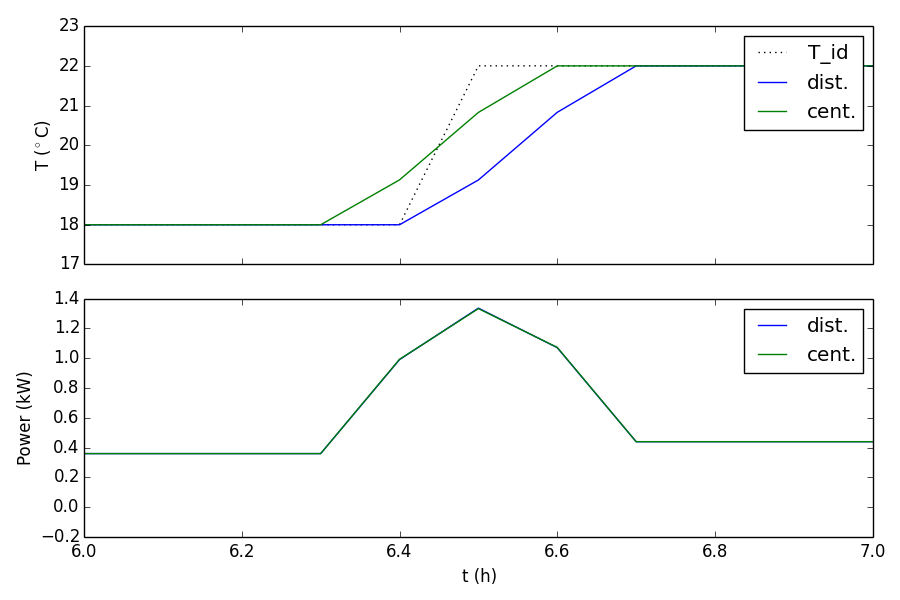
\includegraphics[width=3in]{dynDMPC_initZOOM.png}
\caption{Optimal power distribution in a dynamic case for user 2 in a symmetrical problem, focus between 6\hc 30-8\hc 30 am
\rem{j'ai l'impression que le décalage de la courbe bleue est un bug de programme ou de notation (décalage d'indice temporel).
Dans tous les cas, la superpotion de ces courbes n'est pas très intéressante, car c'est juste un diagnostic pour dire ``DMPC marche comme MPC centralisé. N'en garder qu'une ?}
}
\label{dynDPBinit}
\end{figure}

As before, we now consider a situation where user 2 is preferred and has a comfort factor ten times superior to others. 
 
\begin{figure}[H]
\centering
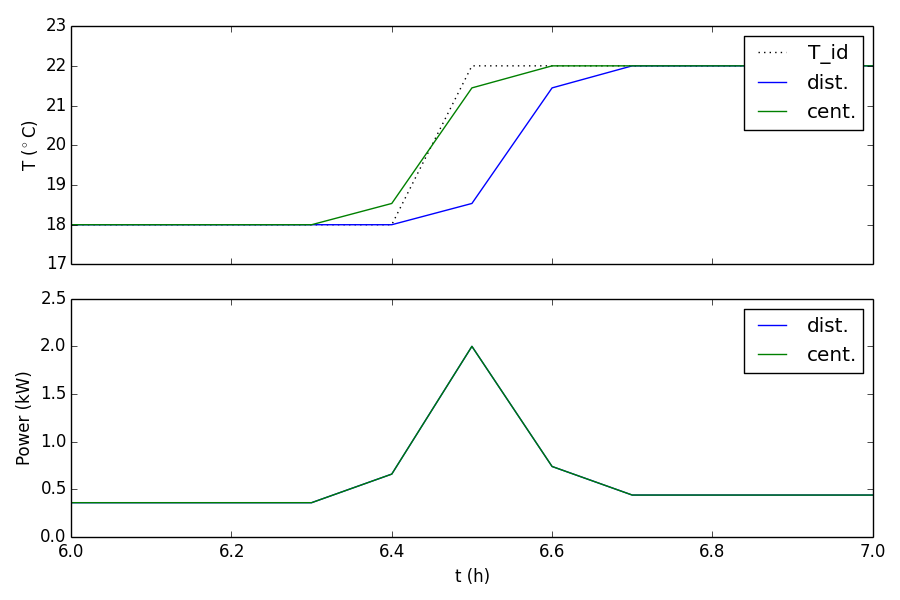
\includegraphics[width=3in]{dynDMPC_chtZOOM.png}
\caption{Optimal power distribution in a dynamic case for user 2 when it is preferred, $\alpha_2 / \alpha_0 = 10$, focus between 6\hc 30-8\hc 30 am
\rem{rem. idem fig. 8}
\rem{par contre là on aimerait bien voir, superposés, le profil de température pour les deux utilisateurs}
}
\label{dynDPBcom}
\end{figure}
 We notice comparing Figures \ref{dynDPBinit} and \ref{dynDPBcom} that in the second case, user 2 is given mush more energy when needed and hence can reach its ideal temperature much faster.

From this point on, we are able to use this model to begin the study of cheating and misleading scenarios.
  
\section{Security issues : misleading and cheating users}
In this section, we will focus on the security issues of the DMPC. First, we will analyse the different ways of cheating before putting it into application on static and then dynamic situations. 

\subsection{Security concepts}

PH: {\itshape très bien d'introduire comme ça. Je pense que le texte et le diagramme (fig 10) méritent qq reformulations pour clarifier les concepts. ''greedy`` et ''nihilist`` sont expliqués, mais pas le niveau de dessous (''structural``, ....)

Par ailleurs, il faudrait clarifier ce à quoi l'attaquant a accès: un sous contrôleur, plusieurs, le coordinateur ?
Je crois que l'étude focalise sur la modification d'un sous contrôleur.
}

First of all, we must clarify the concept of security breach in a DMPC. Through our research, we were able to detect two kinds of threatening users : greedy users (whose objective is to maximize their comfort) and nihilist users (whose objective is to destroy the system). 

 \begin{figure*}[!t]
\centering
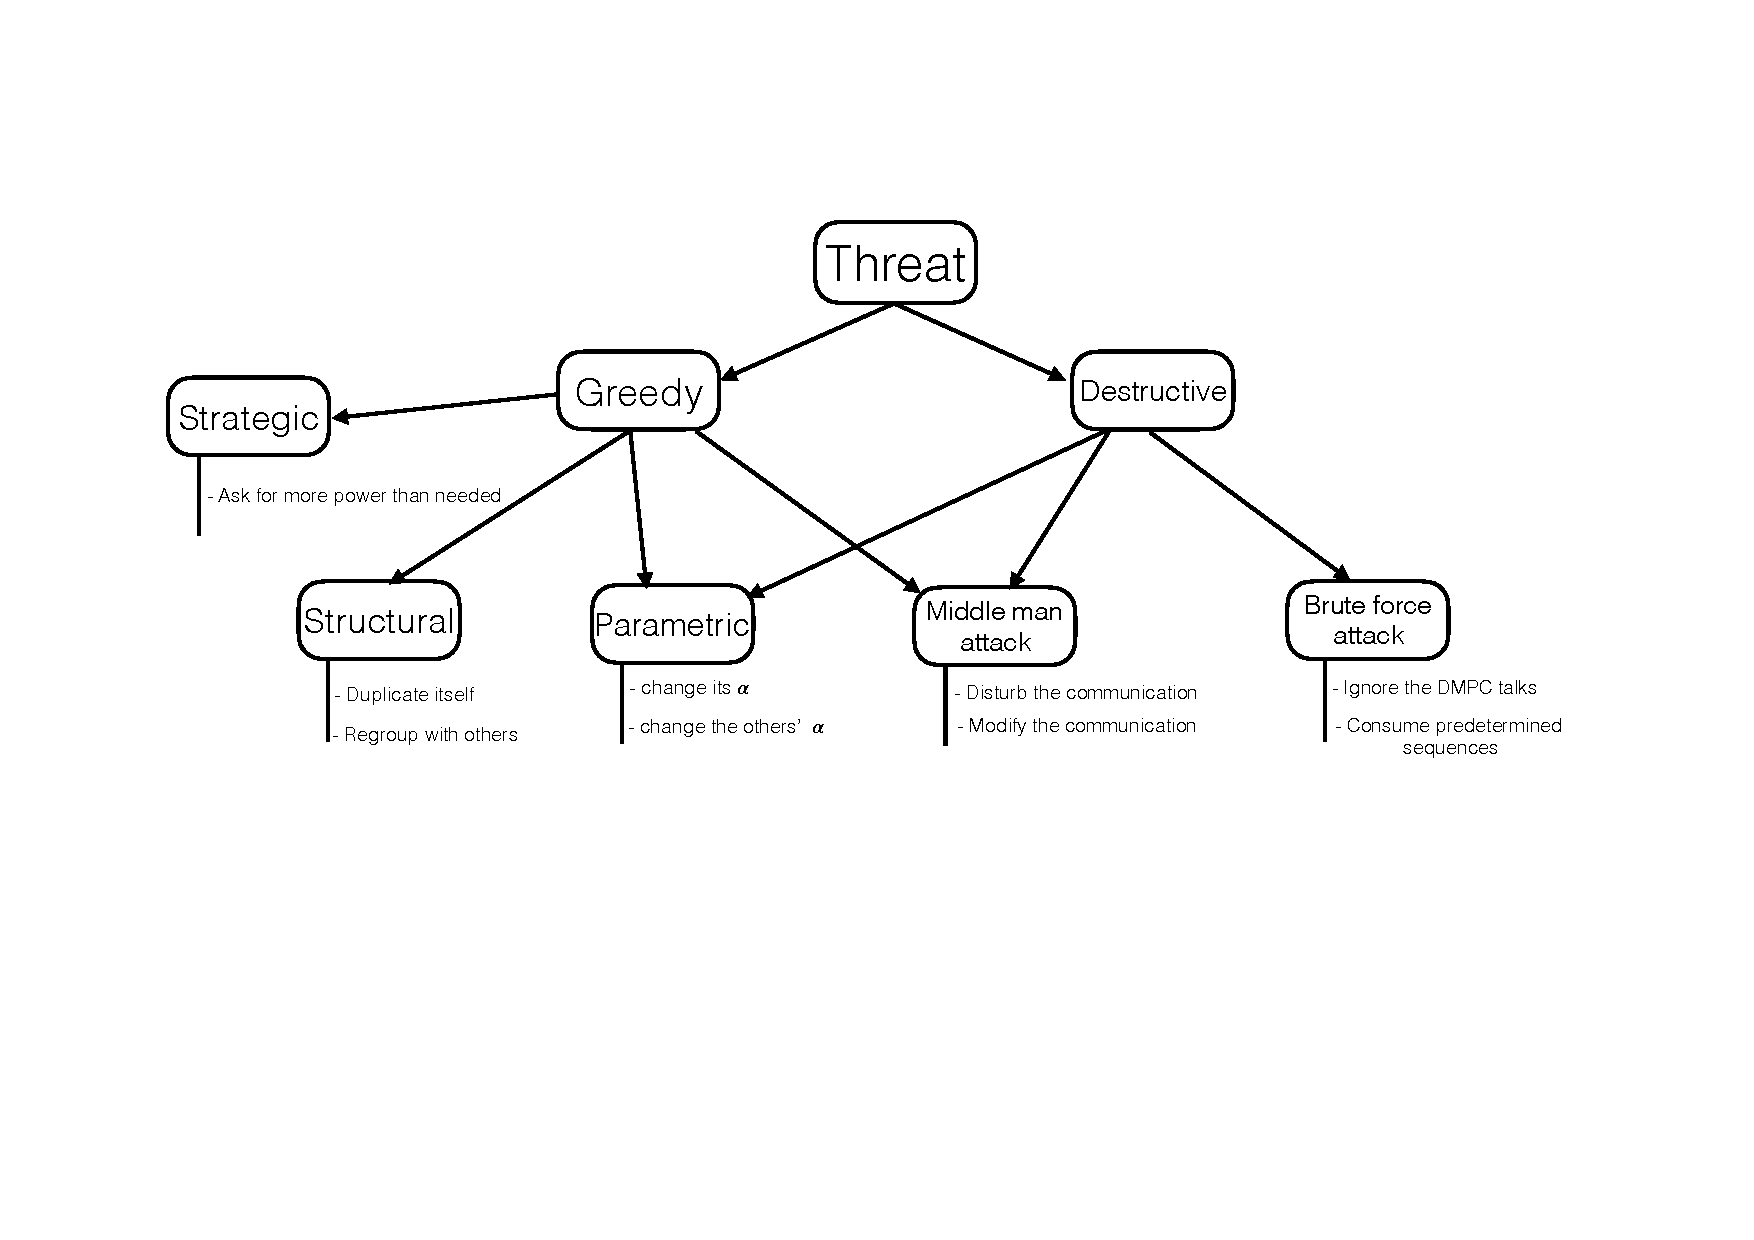
\includegraphics[width=5.5in]{mindmap}
\caption{Overview of different attack methods
\rem{bonne structure, affiner le texte}
}
\label{mindmap}
\end{figure*}

In Figure \ref{mindmap}, we can see an overview of the different threat we detected. The reader can note that even if other strategies might exist, we realized  that all the other strategies can be somehow reduced to one of those we studied. 

Moreover, for our study we considered that the transmission canal is ideal and that the communication cannot be altered. Indeed with the current knowledge, security protocols enable us to safely communicate and to change ones identity. This implies that in our model cheating by usurping ones identity or by altering the communication is not considered. Moreover, unless the demand profile of the users are complementary, the strategy of regrouping is ineffective. \\

To summarize, the base threatening \rem{threatening = menaçant ? Préférer attack?} cases are as follow :
\begin{itemize}
\item[•] Change its own comfort factor $\alpha_i$.
\item[•] Change its broadcasted ideal temperature. \rem{n'apparait pas comme tel sur fig 10}
\item[•] Do not listen to the DMPC talks. \rem{''talks`` → ''negociation`` ? Préciser peut être : ''Uzawa iterations to satisfy the global power limitation``?}
\item[•] Listen partially to the DMPC talks. \rem{préciser ''takes in its local optimization only a \emph{fraction} of the multiplier $\lambda$. see details in next section`` ?}
\item[•] Duplicate itself.\rem{idée qui mérite une explication}
\end{itemize}

\subsection{Security in static situations}
Now, we implement those strategies into the static model. 
\rem{Explain why.}

\rem{cette partie peut éventuellement être coupée en 3 \texttt{subsubsections}}

First, we implemented the influence of the comfort factor $\alpha$. The idea was to determine to which extent this parameters changes the power distribution. In figure \ref{SCHT_a2}, we represent the optimal power distribution and the temperature deviation for two users \rem{cohérence avec les figures 3-6: ça serait mieux d'avoir 3 utilisateurs pour retrouver les valeurs numériques d'une expérience à l'autre} when the comfort factor is a parameter. We noticed that, as expected, when the one user comfort factor is superior to the one of the others,  it receives much more energy and as therefore a better comfort. In figure \ref{SCHT_a5}, we notice that the more users there are against a user who changes its comfort factor, the more they are neglected in regard to the cheater.\rem{là je suis pas vraiment d'accord, car je crois que Umax n'a pas été mis à l'échelle !}

\begin{figure}[H]
\centering
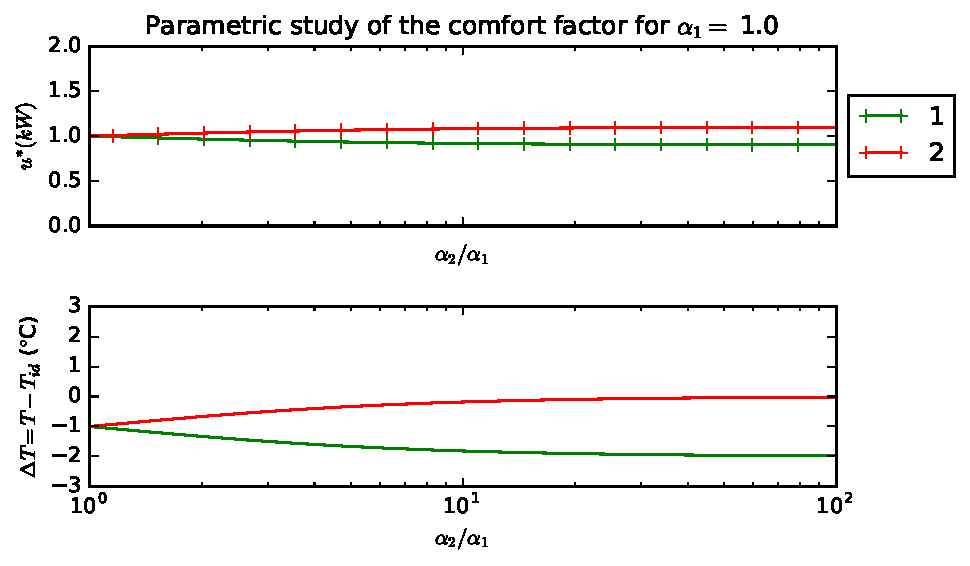
\includegraphics[width=3in]{statcht2alpZ.pdf}
\caption{Parametric study of the comfort factor for two users}
\label{SCHT_a2}
\end{figure}

\begin{figure}[H]
\centering
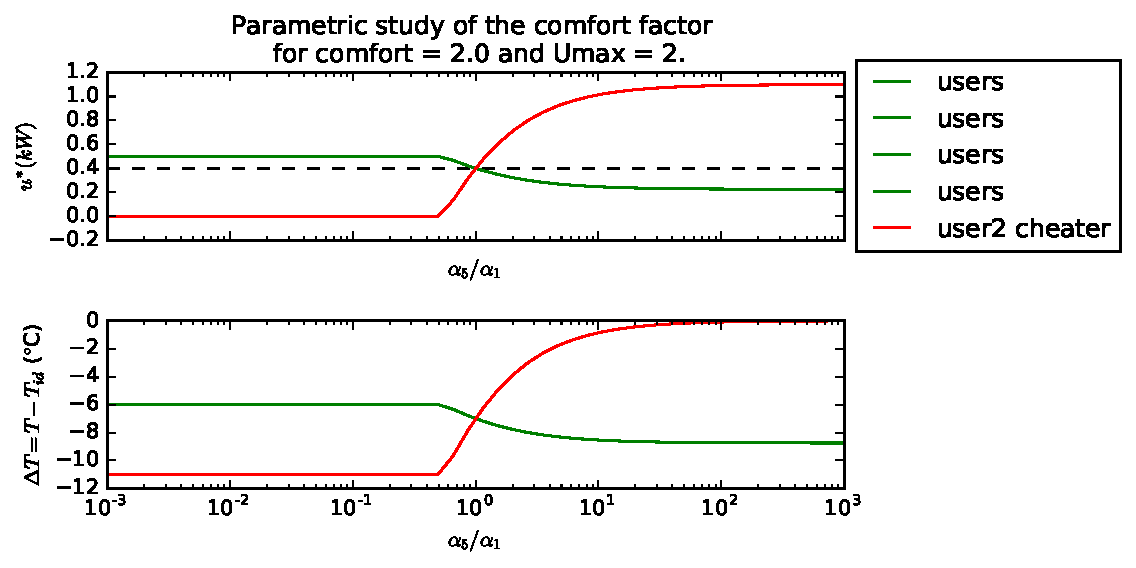
\includegraphics[width=3.5in]{statcht5alp.pdf}
\caption{Parametric study of the comfort factor for five users
\rem{Cohérence : échelle horizontale très différente entre fig 11 et fig 12. de même que le titre}
}
\label{SCHT_a5}
\end{figure}

Then, we determine the influence of the broadcasted
\rem{enlever ''broadcasted`` car c'est u qui est transmis au coordinateur. Tid est interne à chaque contrôleur.}
ideal temperature on the distribution. In Figure \ref{SCHT_T} is represented the power distribution and the temperature deviation as functions of the broadcasted temperature. We notice that the higher this temperature is, the more energy the user receives and the less its deviation is. Please note that in our model if a user receives energy, this user has to consume it (hence the positive deviation in Figure \ref{SCHT_T}).
\rem{conclure sur le fait que cette stratégie est donc piège pour celui qui l'utilise}

\begin{figure}[H]
\centering
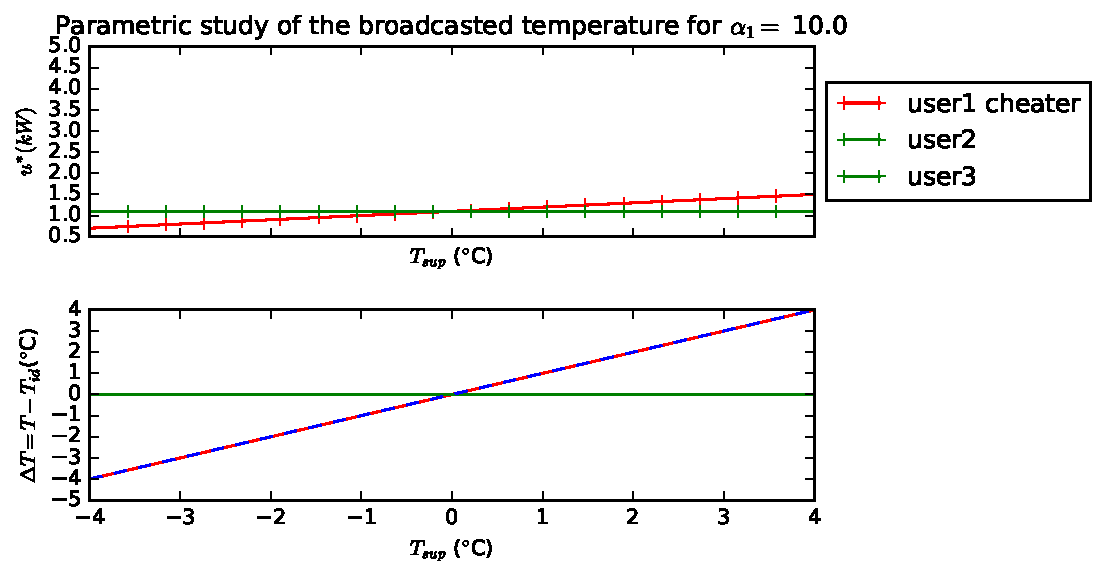
\includegraphics[width=3.5in]{statchtbcT.pdf}
\caption{Parametric study of the broadcasted ideal temperature when different from the real ideal temperature for three users
\rem{Cohérence avec les autres expériences : pourquoi ici le $Delta T$ de base est 0° alors qu'il vaut -2.7 en fig 1 et -1 en fig. 11 ? → homogénéiser les cas d'études}
}
\label{SCHT_T}
\end{figure}

%\begin{figure}[H]
%\centering
%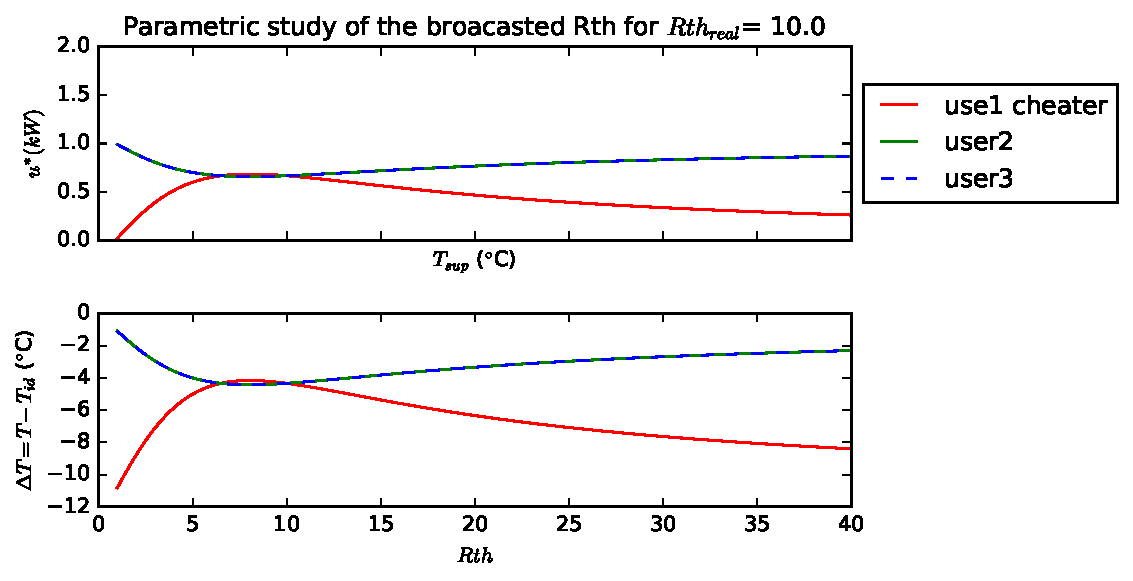
\includegraphics[width=3.5in]{statchtbcRth.pdf}
%\caption{Parametric study of the broadcasted thermal resistance when different from the real $R_{th}$ for three users}
%\label{SCHT_rth}
%\end{figure}

Finally, we created a situation where a user could listen or not to the talks of the DMPC. This means the user can decide if it takes into account the Lagrangian multiplier returned by the coordinator. We introduced this notion as the deafness factor $\beta$. If the user behaves and listen, $\beta = 0$, but if he is deaf,  and does not take the talk into account,  $\beta =1$.
\rem{donner ici la nouvelle définition de la fonction objective locale qui inclut $\beta$}.

In Figure \ref{SRecal_i}, the nominal situation is presented and in Figure \ref{SRecal_} a situation were user 1 is deaf is presented. We do notice that when the user is deaf, its comfort is much better than when it listens to the talk.
\begin{figure}[H]
\centering
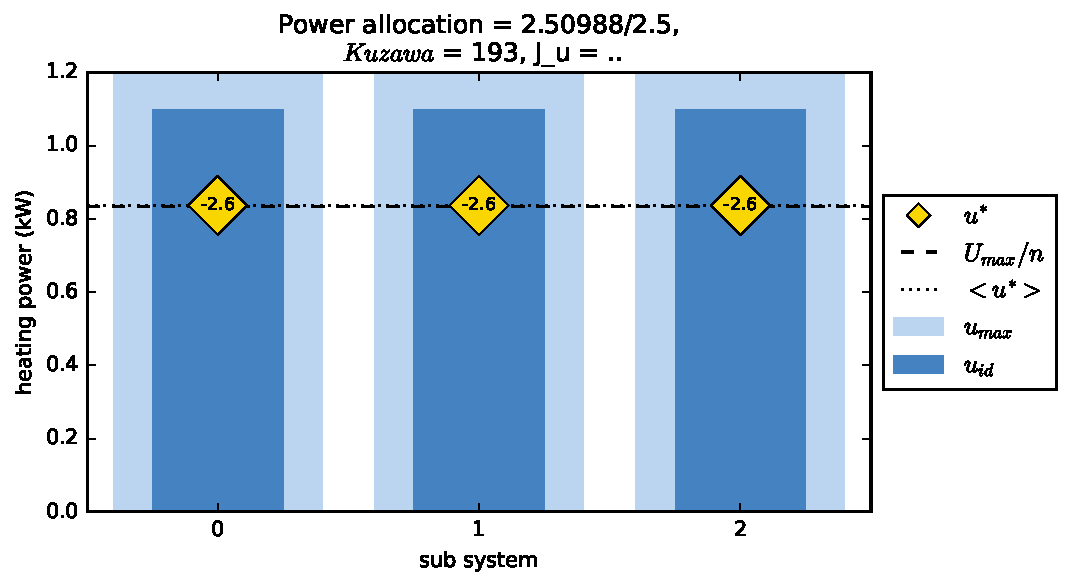
\includegraphics[width=3in]{StatRecal_init.pdf}
\caption{Power distribution for three user in the nominal case
\rem{cohérence avec fig 3-6: ici umax > uid alors que umax < uid dans fig 3-6. Je trouve d'ailleurs que c'est mieux comme ça. → adapter fig 3-6}
}
\label{SRecal_i}
\end{figure}

\begin{figure}[H]
\centering
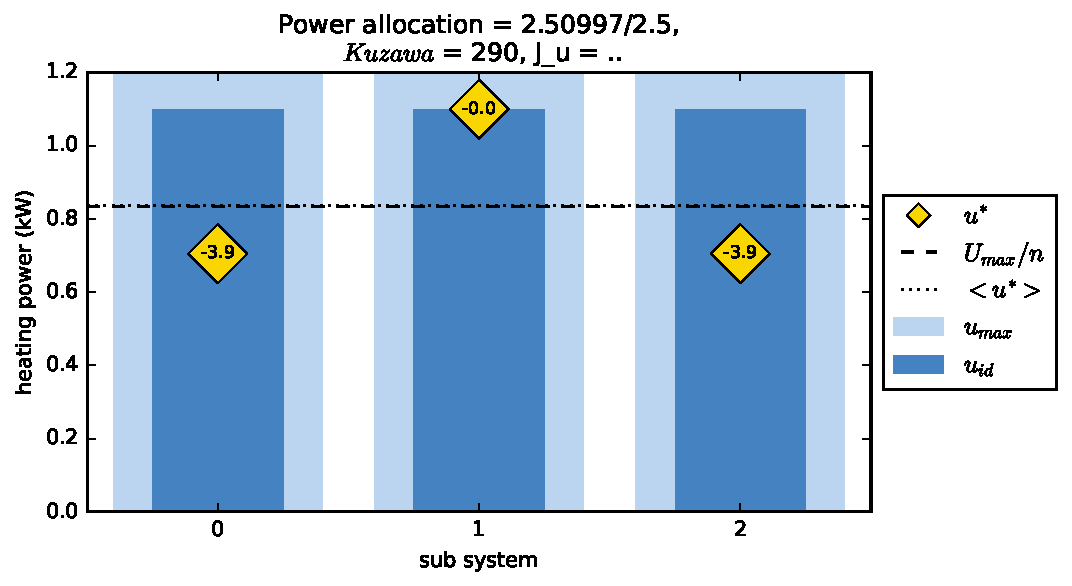
\includegraphics[width=3in]{StatRecal.pdf}
\caption{Power distribution for three users when user 1 does not listen to the talk}
\label{SRecal_}
\end{figure}
Of course this deafness factor $\beta$ can be set between 0 and 1. Figure \ref{SRecal_mult} shows the influence of the deafness factor of user 1 on the temperature deviation of both users. With no surprise, when a user is not listening to the value of the multiplier $\lambda$ (i.e. which penalizes power consumption) all the others are penalized \rem{depreciated s'applique plutôt à des actifs financiers apparemment}.

\begin{figure}[H]
\centering
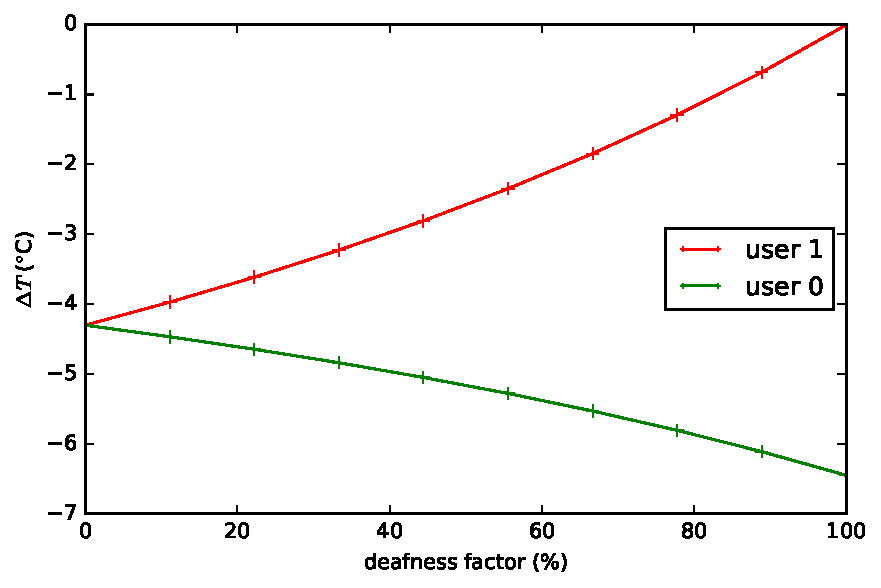
\includegraphics[width=3in]{param_mult.pdf}
\caption{Parametric study of the deafness factor on the deviation to ideal temperature}
\label{SRecal_mult}
\end{figure}

All those studies have been executed on the static model, but all those results can easily be extended to the dynamic model and to the DMPC. 

\subsection{Security in dynamic situations}
Now, let us consider the dynamic model.

\paragraph*{Remark on implementation}
Our current Python simulation module implements both centralized MPC and distributed MPC. However, due to the Uzawa iterations of DMPC, its simulation requires much more computation time (factor 100 or more).
As a consequence, the numerical results of this part are obtained with
the centralized MPC implementation. However, they still represent a distributed system and as such these results should be reproducible with a real DMPC implementation.

\subsubsection{First, we consider a cheating user}
We want to observe the influence of the comfort factor. In figures \ref{DMPCa_1} and \ref{DMPCa_2} we can observe the situation with two users. In blue we can see the distribution in the nominal case were $\alpha_1=\alpha_2 = 10$. Then we change the value of the comfort factor for the second user. We notice that its comfort is drastically better (follows the reference temperature more than the green and the blue lines) to the detriment of the first user (in green).

\begin{figure}[H]
\centering
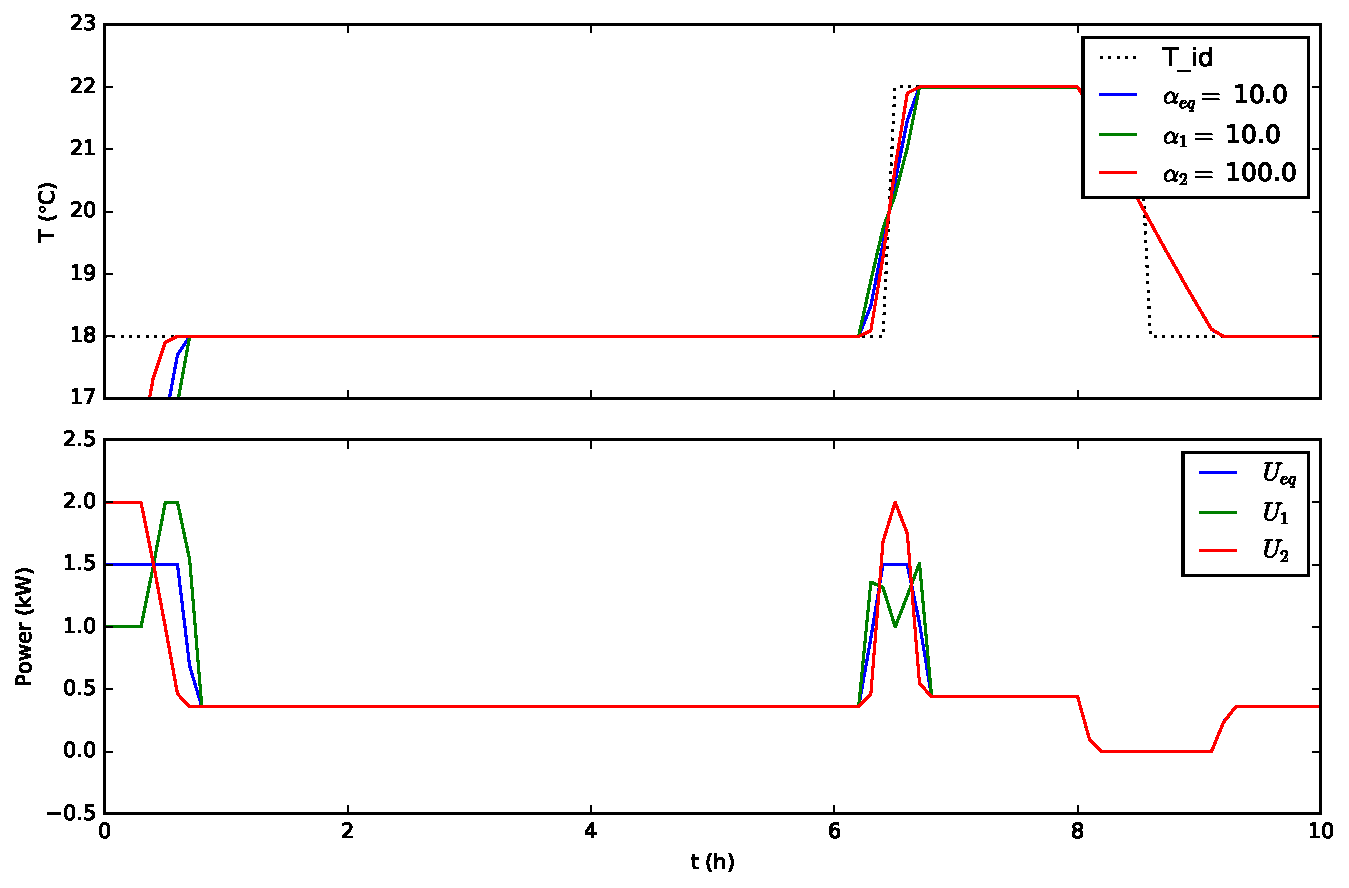
\includegraphics[width=3in]{DMPCalp.pdf}
\caption{Power distribution through time for two users. In blue is the nominal situation with identical comfort factor.}
\label{DMPCa_1}
\end{figure}

\begin{figure}[H]
\centering
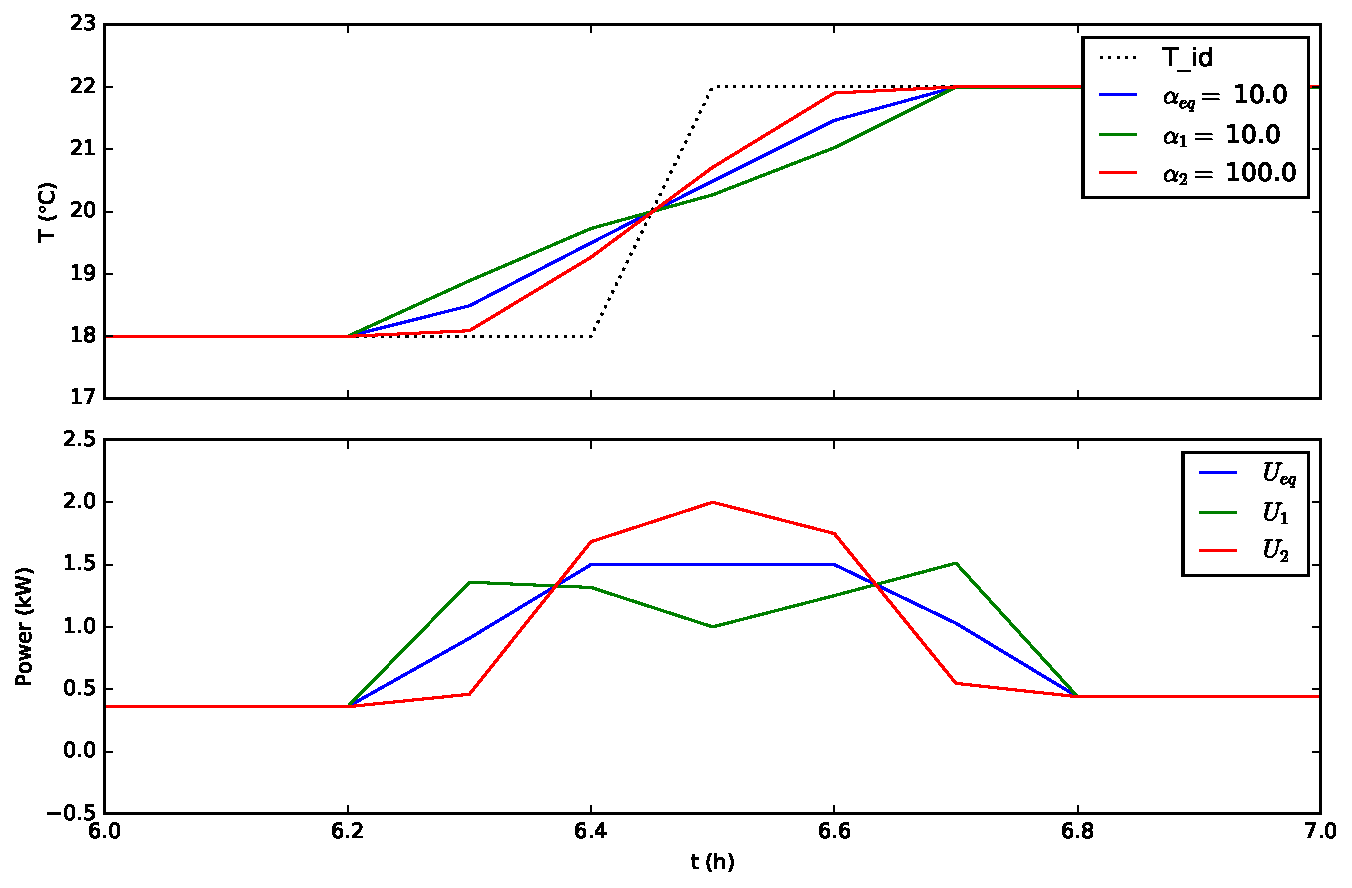
\includegraphics[width=3in]{DMPCalpZ.pdf}
\caption{Power distribution through time for two users. In blue is the nominal situation with identical comfort factor. Focus between 6\hc 00-7\hc 00 am
\rem{je trouve ce graph très clair (sauf font trop petite)}
}
\label{DMPCa_2}
\end{figure}

Our study pointed out that the more $\alpha_2 > \alpha_1$, the more user 2 has a great comfort and the opposite for user 1. Hence, by modifying $\alpha$, one could easily cheat the DMPC in order to gain access to more energy.


\subsubsection{Then, we consider a nihilist user.}
As previously stated, a nihilist user is a user whose objective is to disrupt the system and even destroy it. In our first subsection, we presented several strategies in order to disable the DMPC system.  During this phase, we evaluated the influence of different parameters to detect if they could be a liability in the DMPC. We notice that by augmenting the comfort factor of all users, we could reach a threshold and make the Uzawa iteration not converging (or at least reaching the maximum admissible iteration $k_{max}$). Hence if a user succeeds to change the value of all the $\alpha$, it might be able to break the DMPC. 

Secondly, we tried the other method : to use a specific, custom-made, sequence $u^*_i[k]$ \rem{là encore clarifier qui est ce $k$. ça se complique par le fait qu'on est dans le cas dynamique...} instead of the result of the local optimization. We created a sequence such as $u_2[k] = u^i_{max}$ if k is an odd number and  $u_2[k]=0$ else.  In Figure \ref{Nihil_1}, we show the distribution through time for the non-nihilist user (user 1). In Figure \ref{Nihil_2}, we show the same but for the nihilist user (user 2).
\begin{figure}[H]
\centering
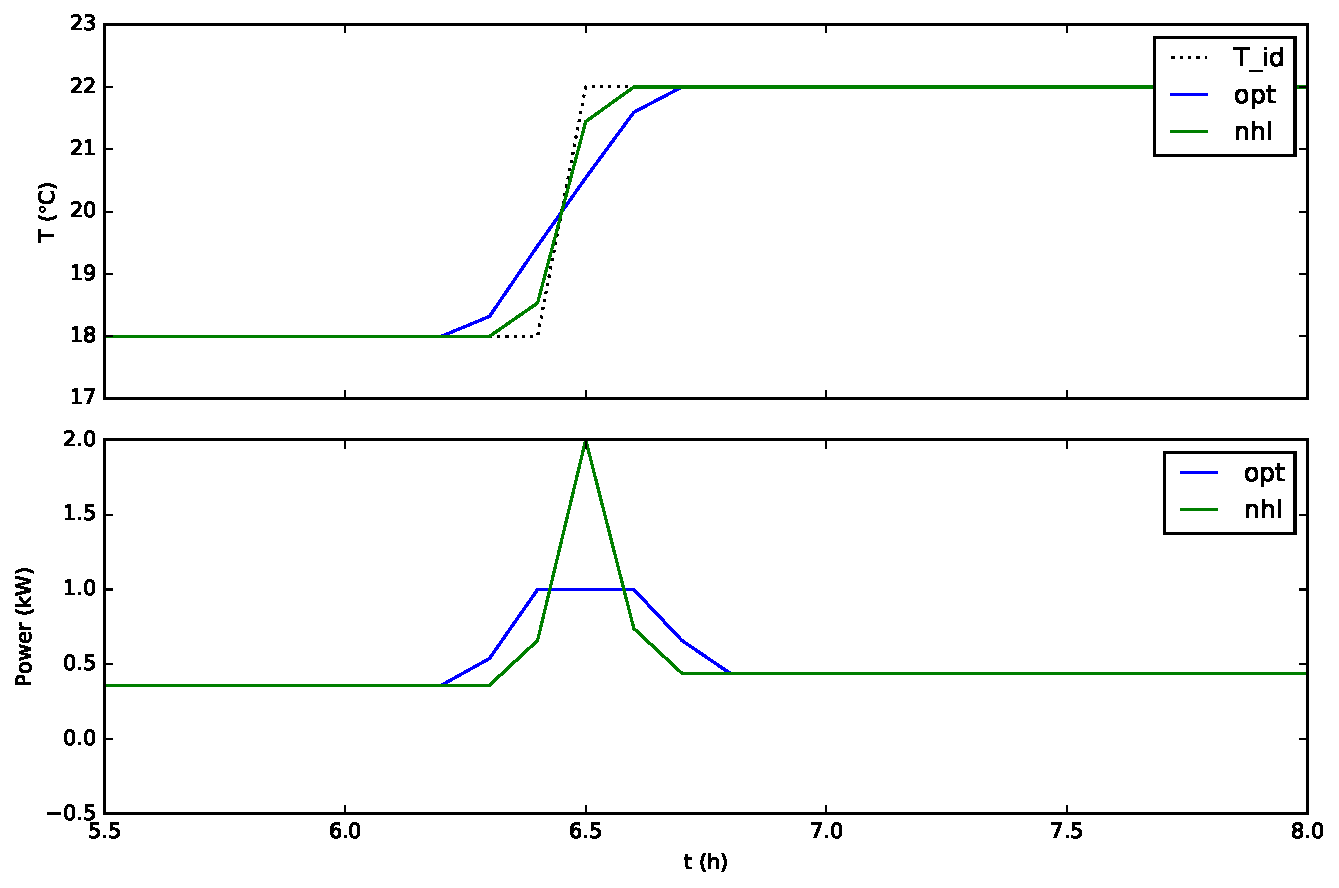
\includegraphics[width=3in]{NihilSeq_init.pdf}
\caption{Power distribution through time for user 1 when applying a destroying sequence of consumed power for user 1}
\label{Nihil_1}
\end{figure}

\begin{figure}[H]
\centering
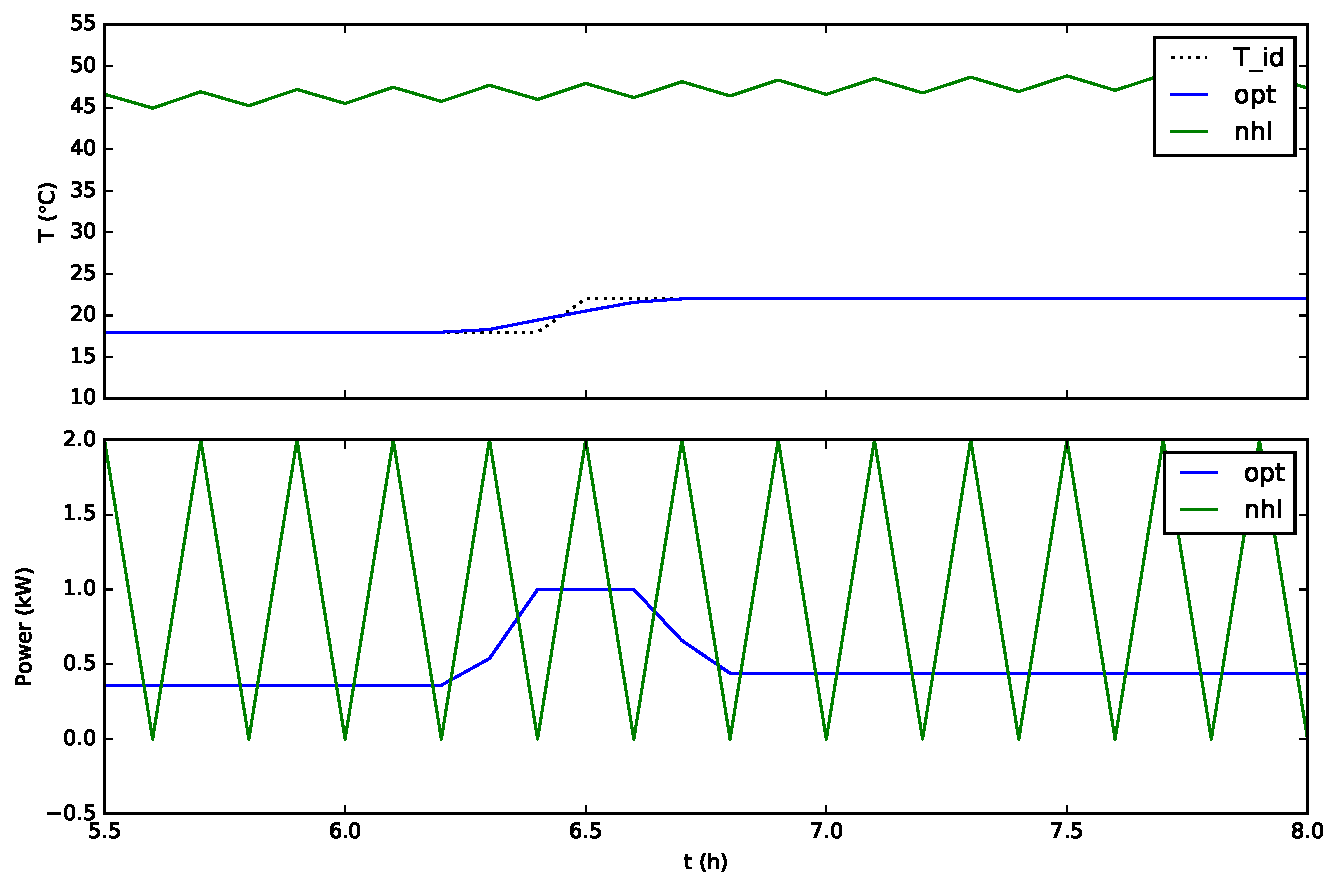
\includegraphics[width=3in]{NihilSeq.pdf}
\caption{Power distribution through time for user 0 when applying a destroying sequence of consumed power for user 1
\rem{je comprends pas pourquoi user 0 est à ce point perturbé par user 1. Sa température devient très grande. ne serait-ce pas le graph de user 1?}
}
\label{Nihil_2}
\end{figure}

When summing $u^*_1$ and $u^*_2$ we notice that the max is superior to the amount of energy available $U_{max}$. This proves that this sequence disable the DMPC. 

\subsection{Protection}
Finally, we studied security counter-measures against those threat. We noticed through our experiment that when we were altering the parameters, we modified as well the following functions :
\begin{itemize}
\item[•] $k_{Uzawa} \rightarrow (u^*(k_{Uzawa}) | \alpha)$
\item[•] $\lambda \rightarrow (u^*(\lambda) | \alpha)$
\item[•] $k_{Uzawa} \rightarrow (\lambda (k_{Uzawa}) | \alpha)$
\end{itemize} 

\rem{clarifier notation. Le ''sachant $\alpha$'' est hard à lire. Peut être dire plus simplement, en toute lettres, que l'on étudie la grandeur Y en fonction de la grandeur X, pour un certain nombre de valeurs du paramètre Z ?}

In other words, the first (\textit{resp.} second) function represents the power distribution (of one user for a given $\alpha$) as a function of the number of iteration realized in the Uzawa method (\textit{resp.} the value of the Lagrangian multiplier). Similarly, the third one returns the value of the Lagrangian multiplier as a function of the number of iteration realized in the Uzawa method. 

In figure \ref{CM_1}, we can observe the nominal situation. Then in figure \ref{CM_2} we can see a cluster of lines created for different values of $\alpha$.
\rem{pas clair pour moi ce que fig \ref{CM_2} et \ref{CM_3} représentent. Un des points à expliquer est : pourquoi les lignes ne s'arrêtent pas après que Umax/n est atteint. C'est qu'on n'est plus entrain de faire Uzawa mais une analyse paramétrique ? Ou bien que le critère d'arrêt d'Uzawa est désactivé ? }
\rem{Rem sur le  3e subplot de fig 22 : est-on bien sûr que le tracé $\lambda(k)$ ne dépend pas de $\alpha$? Si oui, il faut le commenter}


\rem{paragraphe à ajouter sur la description de ce qu'on voit sur les figures 21-23: 1) diminution de u* avec $\lambda$, effet de plateau au début....}

\begin{figure}[!t]
\centering
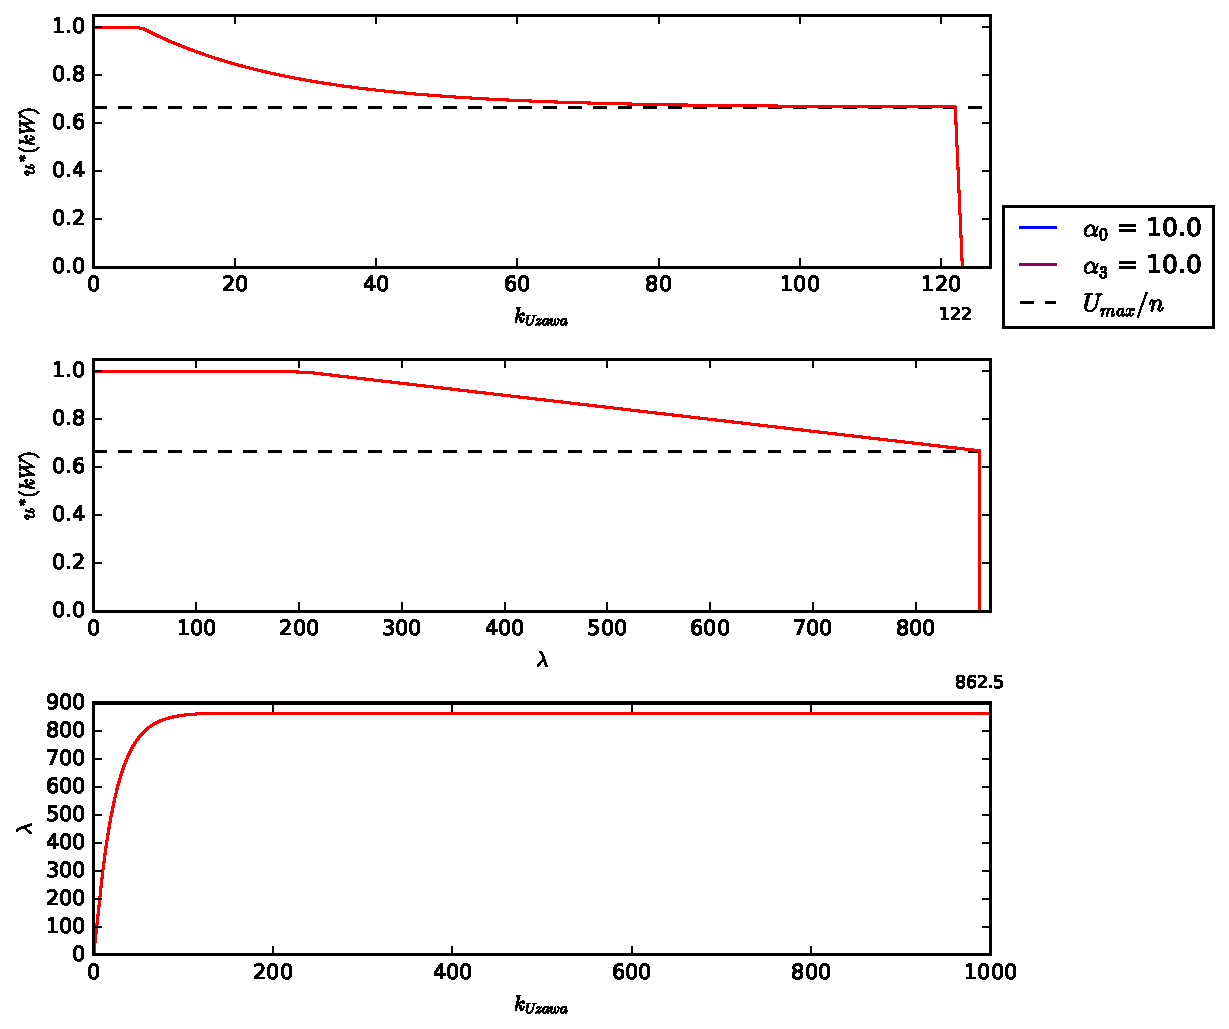
\includegraphics[width=3in]{KL_init.pdf}
\caption{$u^*(k)$, $u^*(\lambda)$ and $\lambda(k)$ in nominal situation. \rem{expliquer que la chute à 120 correspond à la convergence de Uzawa. Dans l'idéal la courbe devrait juste s'arrêter à 0.6, pas tomber à 0 (qui est juste un produit de la pré-initilisation du vecteur ?)}}
\label{CM_1}
\end{figure}

\begin{figure}[!t]
\centering
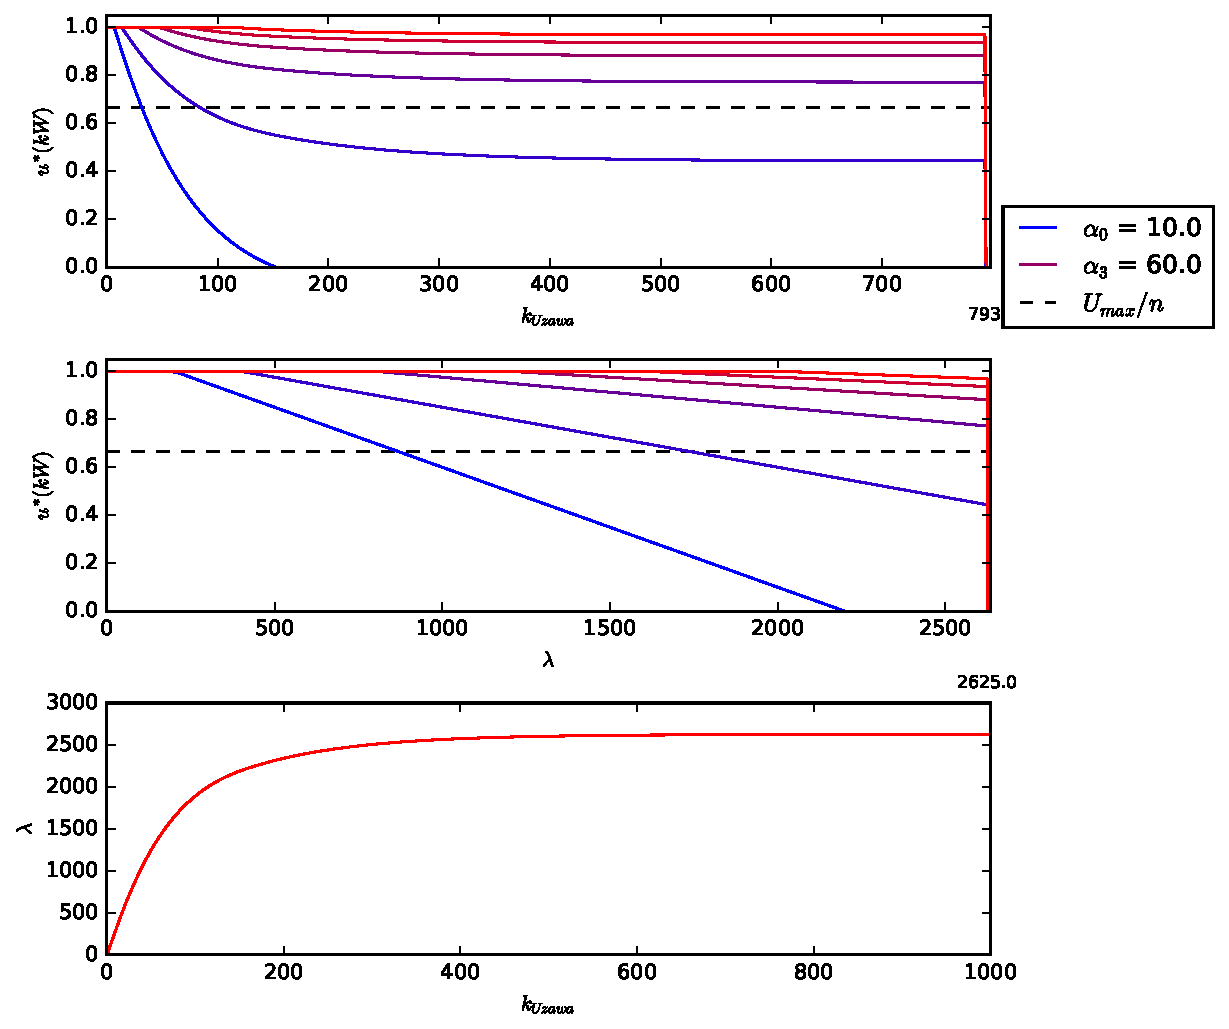
\includegraphics[width=3in]{KL_10-80.pdf}
\caption{Parametric study of the influence of the comfort factor on different functions \rem{remplacer ``functions'' par une description courte de ce qui est représenté}. Comfort factor $\alpha_i \in {10, 20, 40, 60, 80, 100}$.}
\label{CM_2}
\end{figure}

We then decided to realize a large cluster of lines for alpha linearly distributed. The result is presented in Figure \ref{CM_3} for $\alpha$ in range 0 to 150.
\rem{Il me semble il y a voir de la redondance entre fig 22 et 23. Peut-être n'en garder qu'une ?}

\begin{figure}[!t]
\centering
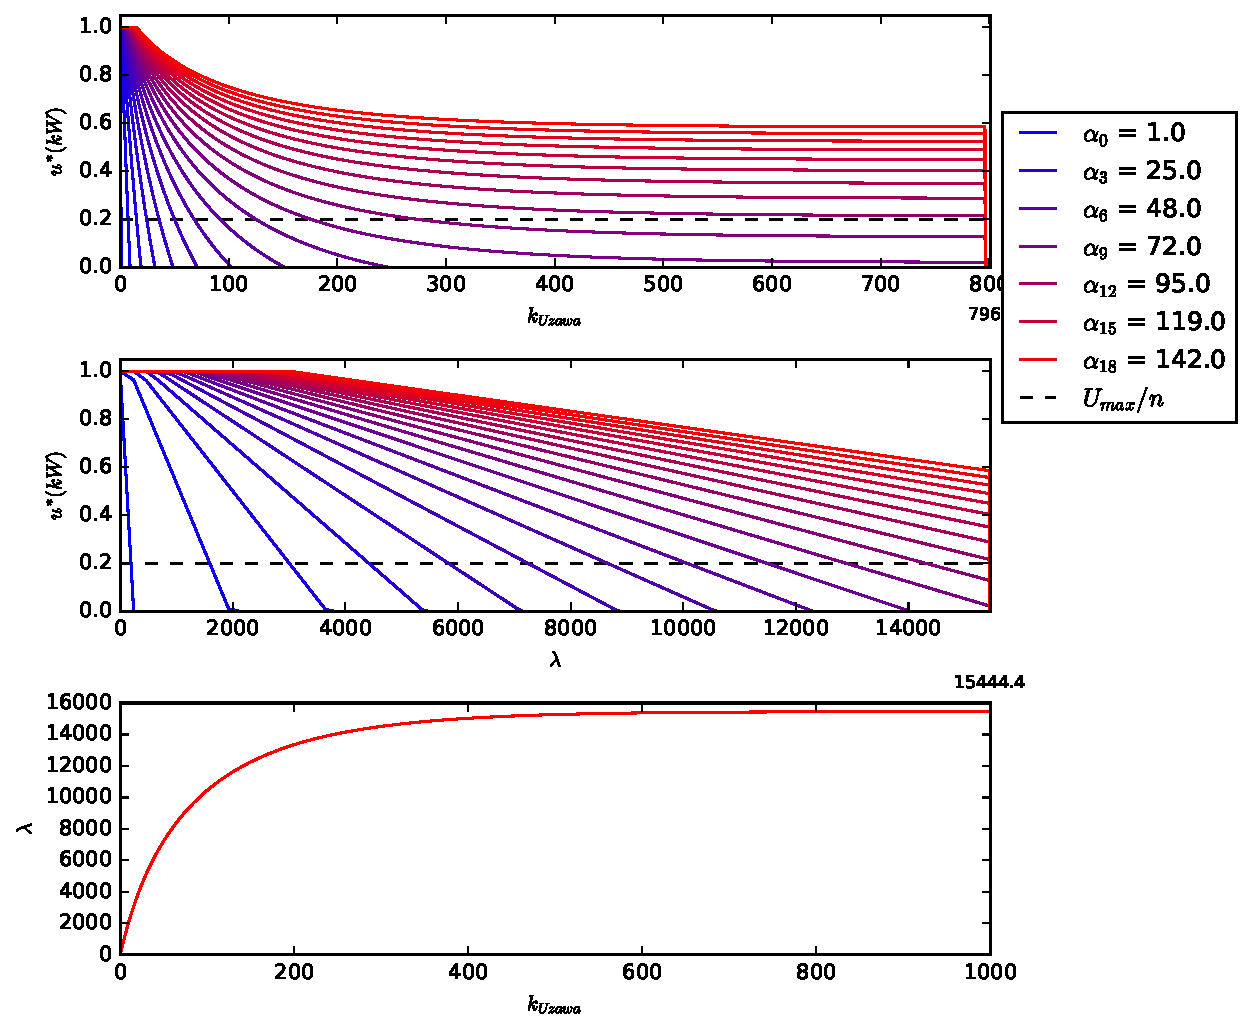
\includegraphics[width=3in]{KL_lin.pdf}
\caption{Parametric study of the influence of the comfort on different functions. Linear distribution of comfort factor.
\rem{pas clair qui sont les $\alpha_1$ ... $\alpha_{18}$ de la légende. Il n'y a pas 18 sous systèmes ?}}
\label{CM_3}
\end{figure}

Thanks to Figure \ref{CM_3}, we can set a threshold (for instance on the line $\alpha_{12}$), this will divide the space in two : above the line $(u^*(k_{Uzawa}) | \alpha_{12})$, user will be considered as cheaters, else the users are cleared. Respectively below the line $(u^*(\lambda) | \alpha_{12})$, user will be considered as cheaters, else the users are cleared.
\rem{ça peut valoir de coup de représenter cette limite sur un graphique par un trait bien visible (genre linewidth=3, alpha=0.5 et une couleur qui tranche). Éventuellement, pour que ça ressorte bien, ça peut être une copie de la figure 23 où la couleur rouge-bleu du faisceau de courbe serait remplacé par du gris.}

This is a way to detect efficiently cheating and nihilist users using a comfort variation approach.  


\section{Conclusion}
In this paper, we presented new results on security breach and measures for distributed model predictive control. By developing a thermal model we were able to experiment various approaches on,  firstly,  how to destroy or cheat, and secondly on how to detect such behaviours. By analysing all  the different method, we managed to reduce those situation to a few base cases much easier to analyse and export to other situations. All those results are encouraging and call for further investigation on the subject. 

\bibliographystyle{ieeetr}
\bibliography{biblio_BSCa}
\rem{je crois que dans réf [3] il manque le journal ou la conf. Le reste est nickel}


\end{document}


